% !TeX document-id = {5f9589b8-498a-4233-98c1-605de3ca7afa}
% !TeX TXS-program:compile = txs:///pdflatex/[--shell-escape]


\documentclass[12pt, paper=a4, bibtotoc, toc=listof, headsepline=true, numbers=endperiod]{scrreprt}

\usepackage[a4paper, includeheadfoot, %bindingoffset=3cm, 
left=3.5cm, right=2.5cm, top=1.5cm, bottom=1.5cm, headsep=0.8cm]{geometry}



%Header
\usepackage[automark]{scrpage2}
\pagestyle{scrheadings}
\clearscrheadfoot
\ohead{\rightmark}
\cfoot[\pagemark]{\pagemark}
\renewcommand*{\chaptermarkformat}{}
\renewcommand*{\headfont}{\normalfont}


%\setlength{\headheight}{12mm} % Höhe der Kopfzeile 




\setheadsepline[text]{0.4pt} % Trennlinie unter Kopfzeile 
%Abstand nach Header Trennlinie
%\usepackage[headsep=5mm]{geometry}

%\setfootsepline[text]{0.4pt} % Trennlinie unter Fußzeile






\setcounter{tocdepth}{3}% Include \subsubsection in ToC
\setcounter{secnumdepth}{3}% Number \subsubsection
\setuptoc{toc}{} % Adds ToC to ToC toDo: remove Pagenumber of ToC in ToC

\usepackage[ngerman]{babel} %Deutsch

\usepackage[utf8]{inputenc} %UTF8 Formatierung

\usepackage[T1]{fontenc}

\usepackage{helvet} %Arial
\renewcommand{\familydefault}{\sfdefault} %Arial

\usepackage{float}
\newfloat{listing}{tbhp}{lst}%[section]
\floatname{listing}{Listing}
\newcommand{\listoflistings}{\listof{listing}{Listing Verzeichnis}}

\usepackage{chngcntr}% http://ctan.org/pkg/chngcntr
\counterwithin{listing}{chapter} %counts chapters of listing




\usepackage[chapter, cache=false]{minted} %Code Formatierung
\newminted{JavaScript}{xleftmargin=\parindent, frame=lines,framerule=0.2pt,framesep=10pt, linenos, breaklines=true, tabsize=3}
\newminted{HTML}{xleftmargin=\parindent,frame=lines,framerule=0.2pt,framesep=10pt, linenos, breaklines=true, tabsize=3}
\newminted{CSS}{xleftmargin=\parindent,frame=lines,framerule=0.2pt,framesep=10pt, linenos, breaklines=true, tabsize=3}
\renewcommand{\theFancyVerbLine}{\sffamily\textcolor[rgb]{0,0,0}{\scriptsize\oldstylenums{\arabic{FancyVerbLine}}}}

\usepackage{caption}
\DeclareCaptionFont{black}{\footnotesize\color{black}}
\DeclareCaptionFormat{listing}{{\parbox{\linewidth-2\fboxsep}{#1#2#3}}}
\setkomafont{captionlabel}{\usekomafont{caption}}




%Caption Listing, Figure Styling
\captionsetup[listing]{labelfont=black,textfont=black} %Caption of Listing
\captionsetup[figure]{labelfont=black,textfont=black} %Caption of Figure

\usepackage{graphicx} %IMG

\usepackage{csquotes}

\usepackage[onehalfspacing]{setspace} %Zeilenabstand


%\usepackage{apacite}
%\bibliographystyle{apacite} 
%%http://www.ctan.org/tex-archive/biblio/bibtex/contrib/apacite/apacite.pdf 
%\bibliography{library} % database is "thesis.bib" located in a "bibtex" subfolder 



\usepackage[
	backend=biber,
	style=numeric,
	sorting=none,
	language=german,
	urldate=comp,
	doi=false
]{biblatex}

\DefineBibliographyStrings{german}{%
	andothers = {et al.},
	and = {\&},
}
\DeclareFieldFormat{url}{\url{#1}}

\usepackage{url}
%\usepackage[draft=false]{hyperref}
\PassOptionsToPackage{hyphens}{url}

\usepackage[anythingbreaks]{breakurl}

\urlstyle{same}

\DeclareNameAlias{}{last-first} %Name in Literaturverzeichnis umdrehen
\DeclareBibliographyDriver{book}{%
	\printnames{author}%
	\setunit*{\addperiod\addspace}%
	\printfield[parens]{year}%
	\setunit*{\addperiod\addspace}%
	\printfield{title}%
	\setunit*{\addperiod\addspace}%
	\printlist{publisher}%
	\setunit*{\addperiod\addspace}%
	\printlist{location}%
	\finentry}

\DeclareBibliographyDriver{misc}{%
	\printnames{author}%
	\setunit*{\addperiod\addspace}%
	\printfield[parens]{year}%
	\setunit*{\addperiod\addspace}%
	\printfield{title}%
	\setunit*{\addperiod\addspace}%
	\printtext{Abgerufen am}
	\printfield{urlday}%
	\setunit*{\addperiod}%
	\printfield{urlmonth}%
	\setunit*{\addperiod}%
	\printfield{urlyear}%
	\setunit*{\newline}%
	\printtext{Abgerufen von}
	\setunit*{\newline}%
	\printfield{url}%
	\finentry}

\AtEveryBibitem{
	
	%	\clearname{translator}%
	%	\clearlist{publisher}%
	\clearfield{isbn} %isbn ausblenden
	\clearfield{doi} %doi ausblenden	
	
}
\addbibresource{library.bib}

%Abkürzungen
\usepackage{acronym}
\renewcommand*{\acffont}[1]{\textit{#1}}
\renewcommand*{\acfsfont}[1]{\textnormal{#1}}


% Neues cite-Kommando oder altes \footcite-Kommando überschreiben
%\DeclareCiteCommand{\smfootcite}[\mkbibfootnote]
%{\usebibmacro{prenote}}                                 
%{\usebibmacro{citeindex}%
%	\setunit{\addnbspace}
%	\printnames{labelname}%
%	\setunit{\labelnamepunct}
%	\newunit
%	\printfield{year}
%}
%{\addsemicolon\space}
%{\usebibmacro{postnote}}


%\renewcommand{\smfootcite}[2][2]{\relax}
\usepackage{pdfpages}


\renewcommand{\labelenumii}{\arabic{enumi}.\arabic{enumii}}
\renewcommand{\labelenumiii}{\arabic{enumi}.\arabic{enumii}.\arabic{enumiii}}
%\pagenumbering{Roman} % Switch Roman

%\title{Konzeption und Entwicklung \\ von adaptiven Web Components}
%\subtitle{Bachelorarbeit}
%\author{im Studiengang \\ Mobile Medien \\ vorgelegt von \\ Christoph Kleber \\ Matr.-Nr.: 26982}
%\date{am \today \\ an der Hochschule der Medien Stuttgart}
%\publishers{Erstprüfer: Prof. Dr. Gottfried Zimmermann \\ Zweitprüfer: Darius Morawiec}


%HEADING Farbe
\usepackage{xcolor}

%\definecolor{headingblue}{rgb}{0.0, 0.48, 0.65}
%\addtokomafont{sectioning}{\color{headingblue}}



\begin{document}

\includepdf{title2.pdf}



\includepdf{erklaerung.pdf}





\chapter*{Kurzfassung}
\addcontentsline{toc}{chapter}{Kurzfassung}
In dieser Bachelorarbeit wird ein relativ junges Themengebiet der \emph{Frontend} Webentwicklung, die \emph{Web Components} behandelt. Parallel wird auf die Problemstellung der adaptiven Webentwicklung, also der Anpassung des Webauftritts an den jeweiligen Nutzer und dessen Präferenzen eingegangen und diese Problemstellung auf die \emph{Web Components} angewendet. Zuerst wird konzipiert, wie sich eine Adaptivität ausdrücken und wie sie umgesetzt werden kann. Hier ist erarbeitet worden, dass Nutzer einen Satz an Präferenzen mit jeweiligem Wert besitzen. Dieser Satz wird gespeichert und beim Aufruf der Webseite abgefragt. Anhand der Werte soll das Aussehen und der Aufbau der Komponenten einer Webseite angepasst werden.
In den Kapiteln der \emph{Web Components} wird zuerst deren Geschichte und Technologie behandelt. Danach wird auf verschiedene \emph{Frameworks} aus diesem Segment eingegangen. Aufgrund der vorhergehenden Ergebnisse der gesamten Kapitel werden dann vorhandene \emph{Web Components} gewählt und diese zur erfolgreichen Adaptivität angepasst. Zuletzt wird evaluiert inwiefern diese Anpassung erfolgen konnte und dass \emph{Web Components}, unter guten Voraussetzungen, zur Adaptivität geeignet sind.
{\let\clearpage\relax \chapter*{Abstract}}
The subject of this bachelor thesis is a relative new topic of frontend web development, the \emph{Web Components}. Parallel the problem statement of adaptive web development, the adaption of a website to its user and his preferences, is addressed and conveyed to \emph{Web Components}. First a concept is designed, how adaptivity can be expressed and implemented. The outcome of this is that users have a set of preferences with a certain value to each preference. This set is saved and requested by invocation of the website. Based on these values the appearance and structure of the website should be adapted. In the chapters about \emph{Web Components} first their history and technology is covered. Subsequently different frameworks of this subject are approached. On grounds of preceding outcomes of all chapters, existing \emph{Web Components} are chosen and adjusted to successful adaptivity. Last it is evaluated how far these adjustments could be ensued and that, under good preconditions, \emph{Web Components} are applicable to adaptivity.



\listoflistings
\listoffigures

\chapter*{Abkürzungsverzeichnis}
\addcontentsline{toc}{chapter}{Abkürzungsverzeichnis}
\begin{acronym}
	\acro{API}{Advanced Programming Interface}
	\acro{DOM}[DOM]{Document Object Model}
	\acro{HTML}[HTML]{Hypertext Markup Language}
	\acro{URL}[URL]{Uniform Resource Locator}
	\acro{HTML5}[HTML5]{Hypertext Markup Language Version 5}
	\acro{CSS}[CSS]{Cascading Style Sheets}
	\acro{W3C}{World Wide Web Consortium}
	\acro{REST}{Representational State Transfer}
	\acro{HTTP}{Hypertext Transfer Protocol}
	\acro{JSON}{JavaScript Object Notation}
	\acro{WCAG 2.0}{Web Content Accessibility Guidelines 2.0}
	\acro{AWC Framework}{Adaptive Web Components Framework}
\end{acronym}

\tableofcontents



\chapter{Einleitung}
%\pagenumbering{arabic} % Switch to normal numbers
Im Folgenden wird der Aufbau dieser Arbeit vorgestellt. Im ersten Kapitel wird der Aufbau der Abhandlung beschrieben. Daraufhin wird im zweiten Kapitel die genutzte Methodik dieser Arbeit beschrieben. Im dritten Kapitel wird auf die Adaptivität eingegangen. Hier wird dieser Begriff und dessen Umsetzung erläutert. Danach wird der Nutzungskontext im Zusammenhang der Adaptivität beschrieben. Im vierten Kapitel wird die Adaptivität einer Internetseite an einen Nutzer konzipiert. Hier werden die \ac{WCAG 2.0} im Zusammenhang mit Präferenzen von Nutzern besprochen und daraus Folgerungen für die Präferenzwerte zur Adaptivität erstellt. Das fünfte Kapitel erörtert die Zusammenstellung dieser Präferenzen. Es wird referiert wie diese aufgebaut sind, gespeichert und heruntergeladen werden können, um dann genutzt zu werden. Das sechste Kapitel behandelt die \emph{Web Components}. Es wird auf die Geschichte, die Technik und die Webentwicklung mithilfe dieser Elemente eingegangen. Das siebte Kapitel berichtet über die \enquote{Polymer} Bibliothek und deren Technik. Das achte Kapitel behandelt das \emph{AWC Framework} und dessen Technologie, insbesondere wie die Adaptivität ermöglicht wird. Im neunten Kapitel werden bestehende Web Components zur Ermöglichung der Adaptivität erweitert. Zu jedem Element wird jeweils die Adaptivität konzipiert und im Programmcode umgesetzt. Das zehnte Kapitel evaluiert die Möglichkeit der Anpassung zur Adaptivität der vorhergehenden Elemente. Das elfte Kapitel beschreibt ein Fazit auf Basis der vorhergehenden Kapitel. 

\chapter{Methodik dieser Arbeit}
Im Folgenden wird die Methodik dieser Abhandlung beschrieben. Sie lässt sich in zwei Bereiche aufteilen, \enquote{Adaptivität} und \enquote{Web Components}.
Beginnend mit dem Bereich \enquote{Adaptivität} wird zuerst vorhandene Literatur gesammelt. Diese besteht zum Großteil aus Abhandlungen, Webseiten, Büchern und insbesondere auch Richtlinien zur barrierefreien Gestaltung. Aus dieser Literatur werden Ergebnisse zusammengetragen und mithilfe von persönlicher Interpretation verdichtet. Dadurch werden Präferenzen zur möglichen Adaptivität von Elementen erstellt und evaluiert.
\newline
Der Bereich \enquote{Web Components} setzt sich aus einem Theorie- und einem Praxisteil zusammen. Im Theorie-Teil wird wiederum vorhandene Literatur gesammelt. Diese besteht aus Abhandlungen und zum großen Teil aus Programmdokumentationen und Anleitungen. Diese wird als Basis genutzt, die Technologien der \emph{Web Components} und mögliche nutzbare \emph{Frameworks} zu erforschen. Mit diesen Technologien und \emph{Frameworks} werden verschiedene Tests durchgeführt und Beispiel-Komponenten erstellt, um die Technologien zu erschließen. Die Ergebnisse, eine Kombination aus der Literatur und der Arbeit am Programmcode, werden daraufhin gesammelt. Der Praxisteil beginnt mit der Sammlung und dem Testen von vorhandenen \emph{Web Components}. Von diesen werden einige ausgewählt um diese zu erweitern. Anhand einer Kombination des Theorie-Teils des Bereichs \enquote{Web Components}, also der Arbeit mit den Technologien, und den aus dem Bereich der \enquote{Adaptivität} gezogenen Schlüsse, werden Folgerungen gezogen wie eine Adaptivität konzipiert und insbesondere wie sie im Programmcode umgesetzt werden kann. Dadurch entstehen bei Gelingen adaptive \emph{Web Components}. Daraufhin werden die Komponenten und der Prozess der Erstellung dieser evaluiert.


\chapter{Adaptivität}
Der Begriff Adaptivität wird in vielen verschiedenen Kontexten genutzt. Die Bedeutung ist somit mehrdeutig und abhängig vom Umfeld. Beispielsweise wird in der Psychotherapie unter Adaptivität im therapeutischen Vorgehen eine \enquote{Grundhaltung [beschrieben], welche die Bereitschaft impliziert, unter stetiger Reflexion der Prozesse von Übertragung und Gegenübertragung flexibel auf die jeweils aktuellen Bedürfnisse des Patienten einzugehen} \cite[S.45]{woeller2014tiefenpsychologisch}. Im Kontext von Datenbanken und der \enquote{Adaptivität an unterschiedliche Anforderungen} wird von Verfahren gesprochen, die \enquote{die Anpassungsfähigkeit an unterschiedliche Anforderungen und damit auch an verschiedene Einsatzumgebungen [erhöhen]} \cite[][S.112]{loeser2013web}.
In der Softwareentwicklung kann Adaptivität folgendermaßen beschrieben werden: \enquote{Interaktive Softwaresysteme werden von Benutzern mit unterschiedlichsten Zielen, Interessen, Fähigkeiten, Erfahrenheitsgraden und Präferenzen verwendet. Um einem möglichst breitem Personenkreis zugänglich zu sein, bieten viele derzeit erhältliche Programme bereits die Möglichkeit, daß Benutzer (oder Systemadministratoren) in bestimmtem Ausmaß eine Anpassung des Programms an die jeweiligen individuellen Präferenzen vornehmen können} \cite[S.1]{Kobsa1993}.
\newline In den verschiedenen Auslegungen des Wortes ist ein Muster zu erkennen. Adaptivität kann definiert werden als die Fähigkeit eines Objekts, zum Beispiel eine Person oder ein System, sich an seine Umgebung anzupassen. Diese Anpassung basiert auf bestimmten Einflüssen, so kann sich eine Datenbank an äußere Einflüsse, wie beispielsweise ihre Einsatzumgebung, oder ein Softwaresystem an die Vorlieben seines Nutzers anpassen. Das kann auch automatisch, also ohne aktive Einwirkung des Nutzers, geschehen. So gleicht sich zum Beispiel der Inhalt der Seite \enquote{Facebook} aufgrund eines Algorithmus an den einzelnen Nutzer an, ohne dass dieser bestimmte Einstellungen vornehmen muss \cite{Rixecker2016}. Die Möglichkeit zur Adaptivität kann jedoch auch dem Nutzer bereitgestellt werden. Ist das der Fall, kann der Nutzer beispielsweise die Benutzeroberfläche nach seinen eigenen Vorlieben einrichten. So kann zum Beispiel die Benutzeroberfläche der Entwicklungsumgebung \enquote{JetBrains PhpStorm} anhand persönlicher Präferenzen aufgebaut werden und Farbstile und Kontraste verändert werden.
\newline Hier stellt sich jedoch die Frage, wie im Zusammenhang von Internetanwendungen eine Adaptivität bereitgestellt werden kann und insbesondere, an welche Aspekte sie sich adaptieren soll. Hierfür muss die Umgebung, der Nutzer und auch dessen Arbeitsaufgaben erforscht und definiert werden.
	\section{Nutzungskontext}
	Die Betrachtung des Nutzungskontext bietet diese Möglichkeit. Der Nutzungskontext wird nach der DIN EN ISO 9241-210 von den Benutzermerkmalen, Arbeitsaufgaben und der organisatorischen, technischen und physischen Umgebung bestimmt. Im Folgenden wird ein Überblick dieser Beschreibung gegeben \cite[S.15 ff.]{hoffmann2014venus}.
	\begin{description}  
		\item  [Nutzer und sonstige Interessengruppen] 
		Zu Beginn sollten die Nutzergruppen und weitere Interessengruppen identifiziert und deren wesentliche Ziele und Einschränkungen beschrieben werden.
			
		\item [Merkmale der Nutzer oder Nutzergruppen]
		Diese Merkmale können \enquote{Kenntnisse, Fertigkeiten, Erfahrung, Ausbildung, Übung, physische Merkmale, Gewohnheiten, Vorlieben und Fähigkeiten einschließen} \cite[S.16]{hoffmann2014venus}. Sie beschreiben also insgesamt den Nutzer, um diesen besser einordnen und sich besser an diesen anpassen zu können.
		
		\item  [Ziele und Arbeitsaufgaben der Nutzer]
		Auf der einen Seite werden die Ziele der Nutzer beschrieben, auf der anderen Seite die Gesamtziele des Systems. Danach müssen die Arbeitsaufgaben betrachtet und nach ihren Merkmalen untersucht werden, beispielsweise wie oft eine Aufgabe ausgeführt werden soll.
			
		\item [Umgebung(en) des Systems]
		Die Umgebung lässt sich in die technische Umgebung, also die der Computerkomponenten und Anwendungen, die physikalische Umgebung, also Aspekte wie beispielsweise Beleuchtung und soziale und kulturelle Umgebung aufteilen. Zur kulturellen Umgebung zählen beispielsweise die Arbeitsweise und Einstellungen der Umgebung des Systems.
	\end{description}
	Insgesamt lässt sich somit sagen, dass die Adaptivität an den Nutzungskontext ausgerichtet werden kann. Verschiedene Merkmale des Nutzungskontext haben Einfluss darauf, wie die Adaptivität, passend zur Situation, erfolgen sollte.
\chapter{Adaptivität an den Nutzer}
Nachdem evaluiert wurde an welche Merkmale sich eine Adaptivität anpassen kann wird folgend die Anpassung selbst erläutert. Die Reaktion einer Internetseite, beziehungsweise von deren \emph{Web Components}, die sich adaptiv an den Nutzer anpassen, basiert auf mehreren Schritten. Als Erstes werden Einstellungen und Vorlieben der Nutzer gesammelt und in einer für Maschinen verständlichen Form gespeichert. Der Ort an dem diese gespeichert werden muss immer und von überall erreichbar sein. Als Nächstes müssen die Elemente der Internetseite darauf vorbereitet werden sich anzupassen. Dafür werden Funktionen und Ressourcen bereitgestellt, die bei Bedarf ausgeführt werden oder sich anpassen können. Nachdem dies erfolgt ist, kann die Internetseite, bei Aufruf durch einen bestimmten Nutzer eine Anforderung an den Speicherort stellen, die Informationen des bestimmten Nutzers zu übertragen. Daraufhin wird ein Befehl an alle adaptiven Elemente der Internetseite erteilt. Dieser beauftragt, die Funktionen auszuführen, die zu den jeweiligen Präferenzen und somit Nutzern passen. Dabei verändert sich das Aussehen und unter Umständen der Inhalt der Seite und beweist seine Adaptivität.\newline
Nachfolgend wird in dieser Arbeit darauf eingegangen in welcher Art sich an den Nutzer angepasst werden soll und wie diese Werte gespeichert und abgerufen werden. Als Nächstes wird konfiguriert, wie sich die \emph{Web Components} an die entsprechenden Präferenzen anpassen werden und zuletzt wie das Ergebnis, die adaptiven Elemente einer Internetseite, aussehen wird.
\section{Präferenzen der Nutzer}
Jeder Nutzer hat eigene Vorlieben und Einschränkungen beim Nutzen einer Anwendung. Somit unterscheidet sich die gesamte Nutzerschaft. Um diese Unterscheidung abzubilden werden verschiedene Bezeichner definiert. Jeder Nutzer hat bei jedem dieser Bezeichner einen Wert. Somit wird ein Bezeichner-Wert Paar gebildet. Diese Paare werden gesammelt für jeden einzelnen Nutzer gespeichert. Hierfür werden alle Präferenzen eines Nutzers in einer Zusammenstellung gesammelt und notiert (\emph{Preference Set}).
\section{WCAG Richtlinien}
Um mehr über mögliche Präferenzen in Erfahrung zu bringen werden im folgenden die \ac{WCAG 2.0} Richtlinien betrachtet. Diese versuchen das Internet für alle Personen, unabhängig ihrer Einschränkung, zugänglicher zu machen. Dafür schaffen sie Prinzipien und Richtlinien, auf Basis derer Internetseiten konzipiert werden können. Diese können sehr gut verwendet werden um herauszufinden, in welcher Art und Weise sich Anwendungen adaptiv an verschiedene Nutzer anpassen sollten. Im Folgenden werden die Richtlinien aufgezählt und kurz beschrieben \cite{wcag}.
\begin{description}
	\item [Richtlinie 1.1 Text-Alternativen] Für Texte einer Anwendung sollen nicht aus Text bestehende Alternativen angeboten werden, beispielsweise große Druckbuchstaben, Brailleschrift, Sprache, Symbole oder einfachere Sprache. Parallel dazu sollen nicht textbasierte Inhalte auch durch eine textbasierte Alternative dargestellt werden können.
	\item[Richtlinie 1.2 zeitbasierte Medien] Es sollen Alternativen für Zeit-basierte Medien geschaffen werden.
	\item[Richtlinie 1.3 Anpassbar] Die Möglichkeit den Inhalt der Internetseite in verschiedenen Arten darzustellen, ohne Informationen oder Struktur zu verlieren, soll vorhanden sein.
	\item[Richtlinie 1.4 Unterscheidbar] Den Nutzern soll es erleichtert werden den Vordergrund vom Hintergrund zu unterscheiden. Dies soll bei visuellen und Audio-Elementen kongruent erfolgen. 
	\item[Richtlinie 2.1 Zugänglichkeit mit der Tastatur] Die gesamte Funktionalität der Anwendung sollte auch mit der Tastatur verwendet werden können.	
	\item[Richtlinie 2.2 Ausreichend Zeit] Den Nutzern soll genügend Zeit zur Verfügung gestellt werden um den Inhalt zu lesen und nutzen.
	\item[Richtlinie 2.3 Anfälle] Der Inhalt sollte nicht in der Weise dargestellt werden, die bekannt dafür ist Anfälle auszulösen.
	\item[Richtlinie 2.4 Navigierbar] Es soll den Nutzern ermöglicht werden in der Anwendung zu navigieren, Inhalt zu finden und zu ermitteln an welcher Stelle sie sich befinden.
	\item[Richtlinie 3.1 Lesbarkeit] Der textbasierte Inhalt sollte lesbar und verständlich sein.	
	\item[Richtlinie 3.2 Vorhersehbar] Internetseiten sollen in einer vorhersehbaren Art und Weise auftreten und funktionieren.
	\item[Richtlinie 3.3 Hilfestellung bei der Eingabe] Dem Nutzer soll geholfen werden, Fehler zu vermeiden und zu korrigieren.
	\item[Richtlinie 4.1 Kompatibel] Die Kompatibilität mit heutigen und zukünftigen Benutzeragenten und unterstützenden Technologien soll maximiert werden.
\end{description}
\section{Folgerung für Präferenzen}
\label{sec:folFuePra}
Auf Basis der vorhergehenden Kapiteln, insbesondere den \ac{WCAG 2.0} Richtlinien und weiterer Beobachtungen wird nun erforscht, welche Merkmale eines \emph{Web Component} sich in welcher Art und Weise anpassen sollen, um eine sinnvolle Adaptivität zu erreichen.
\subsection{Kontrast}
Um die \ac{WCAG 2.0} Richtlinie 1.4 zu erfüllen, sollte der Kontrast sich an den Nutzer anpassen. Der Bezeichner Kontrast definiert, ob und inwiefern der Nutzer einen Kontrastwert nutzen möchte, der vom Standard Kontrastwert abweicht. Beispielsweise erleichtert ein hoher Kontrast farbenblinden Nutzern Objekte vom Hintergrund zu unterscheiden. Für Nutzer ohne diese Einschränkung sind zu hohe Kontraste jedoch störend, da sie das Auge schnell ermüden \cite[S.234]{balzert2009webdesign}.
\subsection{Schrift}
Wenn davon ausgegangen wird, dass eine als allgemein lesbar bekannte Schriftart verwendet wird, hat die Wahl einer serifen oder serifenlosen Schriftart keinen bestätigten Einfluss auf die Richtlinie 3.1, die Lesbarkeit eines Textes \cite[S.157-161]{barrierefreiheit}. Jedoch kann, um eine Adaptivität der Schriftart zu ermöglichen, dem Nutzer die Wahl gelassen werden, ob er eine serife oder serifenlose Schriftart nutzen möchte.
Die Schriftgröße kann jedoch Einfluss auf die Richtlinie 3.1 nehmen. So kann eine zu große Schriftgröße, genauso wie eine zu kleine Schriftgröße, die Lesbarkeit beeinträchtigen. Insbesondere älteren Menschen oder Nutzern mit Sehbeeinträchtigungen wird das Lesen eines Textes durch eine anpassbare Schriftart erleichtert \cite[S.152]{barrierefreiheit}. Somit ermöglicht ein Bezeichner Schriftgröße, zu welchem der Nutzer einen Wert wählen kann, eine nützliche Adaptivität der Anwendung. 
\subsection{Leserichtung}
\label{ref:lesRic}
Um die Richtlinie 3.1, die Lesbarkeit, zu erfüllen, sollte die Leserichtung sich an den Nutzer anpassen. Ohne diese Anpassung könnten Missverständnisse und Irritationen entstehen, da Texte von einer anderen Seite gelesen werden. So wird beispielsweise die arabische und hebräische von rechts oben nach links unten, die westliche von links oben nach rechts unten aufgebaut \cite[S.148]{emrich2013interkulturelles}.
\subsection{Anordnung der Elemente}
Kongruent zum Kapitel \ref{ref:lesRic} ist zu bemerken, dass die Sprache des Nutzers und damit seine Leserichtung nicht nur einen Einfluss auf die Texte haben sollte, sondern insgesamt einen Einfluss auf die Gestaltung der Internetseite haben sollte. Aufgrund der Leserichtung fallen Elemente eines Internetauftritts an verschiedenen Stellen unterschiedlich auf. So ziehen bei einer Leserichtung von links nach rechts Elemente in der linken oberen Ecke eher die Aufmerksamkeit auf sich als Elemente in der rechten oberen Ecke, da diese erst danach gelesen werden. Im Gegensatz dazu fallen bei der Leserichtung von rechts nach links Elemente in der rechten oberen Seite schneller auf \cite[S.47 f.]{meidl2013global}.
\begin{figure}
	\centering
	
\includegraphics[width=\textwidth,height=\textheight,keepaspectratio]{leserichtung.png}
	\caption[Einfluss Leserichtung auf Anordnung der Elemente]{Einfluss der Leserichtung auf die Anordnung der Elemente \cite{elShaab} \cite{zeitOnline}}
	\label{img:lesRic}
\end{figure}\noindent
Ein Beispiel dazu bilden die deutsche und ägyptische Nachrichtenseite \enquote{Zeit Online} und \enquote{Al Shaab}, dargestellt in Abbildung  \ref{img:lesRic}. Hier ist im oberen Bereich die Kopfzeile der arabischsprachigen und darunter die Kopfzeile der deutschsprachigen Internetseite abgebildet. Hier sieht man ganz klar, wie im arabischsprachigen Bereich die Elemente eher nach rechts ausgerichtet sind und wichtige Elemente, wie beispielsweise der Name der Zeitung ganz rechts oben angeordnet sind. Im deutschsprachigem Internetauftritt sind die Elemente nach links ausgerichtet und der Name der Webseite ist weit oben links.
\subsection{Text-Alternativen}
Die Richtlinie 1.1 definiert, dass zu jedem Text eine Alternative geboten wird. Darüber hinaus sollen die nicht textbasierten Inhalte nach Bedarf durch einen Text dargestellt werden können. Dem Nutzer sollte ermöglicht werden in seinen Präferenzen anzugeben, ob er den Text oder dessen Alternativen angezeigt bekommen möchte. Dies betrifft bei nicht textbasierten Inhalten vorrangig Steuerungselemente wie zum Beispiel Pfeile in verschiedene Richtungen. Bei Textbasierten Inhalten ist es vom einzelnen Fall abhängig ob ein bestimmter Text durch ein eindeutiges Symbol ersetzt werden kann.
\subsection{Geschwindigkeit}
Die Richtlinie 2.2 sichert dem Nutzer ausreichend Zeit zu, den Inhalt zu lesen und zu nutzen. Dies sollte adaptiv an den Nutzer angepasst werden, da manche Nutzer mehr oder weniger Zeit für eine bestimmte Aufgabe benötigen. Beispielsweise werden bestimmte Navigationselemente durch ein Verweilen der Maus auf diesen ausgeklappt. Sobald die Maus nicht mehr auf dem Element verweilt wird es wieder eingeklappt. Hier sollte es dem Nutzer ermöglicht werden die Zeitspanne anzupassen bevor das Element wieder einklappt, da es ihm andernfalls nicht möglich sein könnte das Element schnell genug zu verstehen und betätigen.
\chapter{Preference Sets}
Die in Kapitel \ref{sec:folFuePra} erarbeiteten Präferenzen betreffen die Nutzer der adaptiven Webseite. Jeder Nutzer hat zu verschiedenen Präferenzen verschiedene Werte. Deshalb ist es notwendig die gesamten Präferenzen jedes einzelnen Nutzers zu speichern um sie später bei Aufruf der Webseite zu nutzen. Diese Sammlung der Präferenzen wird im weiteren Zusammenstellung der Präferenzen beziehungsweise \emph{Preference Set} genannt. 
\section{Speichern der Nutzer Präferenzen}
Die Präferenzen der verschiedenen Nutzer, also die Bezeichner-Wert Paare müssen gespeichert werden. Der Speicherort muss an das Netz angeschlossen sein, da die Werte zur Laufzeit der Anwendung, beziehungsweise beim Laden der Internetseite abgerufen werden müssen. Exemplarisch werden diese über die Versionsverwaltung \emph{Git} auf der Internetseite \enquote{GitHub} gespeichert. Dafür wurde ein \emph{Repository}, also eine Art neues Projekt auf \enquote{GitHub}, mit Namen \enquote{data} erstellt. In diesem werden für einzelne Nutzer und damit deren Zusammenstellung der Präferenzen einzelne  Dateien gespeichert. Diese können dann über eine bestimmte Adresse aufgerufen werden und sind so später beim gewünschten Herunterladen der Präferenzen ansteuerbar. In Listing \ref{lst:jsonPreSet} ist ein Beispiel dieser Zusammenstellung dargestellt.
\begin{listing}
	\begin{JavaScriptcode*}{}
[
	{
		"more-contrast": "true",
		"font-size": "xl",
		"reading-direction": "rtl"
	}
]
	\end{JavaScriptcode*}
	\caption[Beispiel eines Preference Sets]{Preference Set eines Nutzers}
	\label{lst:jsonPreSet}
\end{listing}\noindent
Sie kann über die Adresse 
\newline
\enquote{https://raw.githubusercontent.com/christophkleber/data/master/1} aufgerufen werden. Hier ist zu beachten, dass der einzelne Nutzer durch eine Identifikationsnummer repräsentiert wird, hier die Nummer \enquote{1}. Im späteren realen Gebrauch würde jeder Nutzer eine eindeutige, unter Umständen längere, Identifikationsnummer erhalten. Dies ermöglicht, dass der Nutzer selbst anonym bleibt und dessen Präferenzen nur anhand dieser Nummern abgerufen werden können. Zu jeder vom Nutzer genutzten Präferenz, also dem Bezeichner, wird ein Wert zugeordnet. Beispielsweise ist in Zeile drei zur Präferenz \enquote{more-contrast} der Wert \enquote{true} gesetzt. 
\section{Herunterladen der Nutzer Präferenzen}
\label{sec:herPre}
Um die Präferenzen der Nutzer zu verwenden und auf Basis dieser die Webseite anzupassen, muss eine Möglichkeit geschaffen werden, die Zusammenstellung der Präferenzen beim Aufruf der Anwendung abzufragen. Hierfür wird ein \emph{REST-Client} verwendet. Dieser sendet beim Aufruf der Anwendung einen Befehl an einen bestimmten, an das Netz angeschlossenen, Ort. Dabei wird diesem Ort mitgeteilt, für welche Person die Zusammenstellung angefragt wird. Daraufhin erhält die Anwendung als Antwort alle Präferenzen der mitgeteilten Person und kann auf Basis dieser die Anwendung anpassen.
\subsection{Was bedeutet REST}
Um einen geeigneten \emph{REST-Client} zu erstellen muss genauer auf das \emph{REST} Protokoll eingegangen werden. \ac{REST} ist ein Protokoll um Daten in einer verteilten Umgebung auszutauschen. Es basiert auf den folgenden Prinzipien \cite[S.77]{chauhan2014asp}.
\begin{description}  
	\item  [Adressierbarkeit von Ressourcen]
	Jede Ressource sollte von einem einzigartigen Bezeichner identifiziert werden können.
	
	\item [Einfache und einheitliche Schnittstelle]
	Das \ac{REST} Protokoll basiert auf dem \ac{HTML} Protokoll. Es werden die von der \ac{HTTP}-Technologie bekannten Methoden verwendet. Dies macht das \ac{REST} Protokoll 
	simpel und einheitlich.
	
	\item  [Repräsentation] 
	Die Ressourcen können in verschiedenen Formen repräsentiert werden. Bei Änderung oder Anfrage der Ressource wird immer eine Repräsentation genutzt. Somit kann in einer Anfrage definiert werden, in welcher Form der Repräsentation die Antwort erfolgen soll.
	
	\item [Zustandslos]
	Es werden keine Zustände auf dem \emph{Server} gespeichert. Zustandsinformationen werden vom \emph{Client} gehandhabt und bei Bedarf an den Server gesendet.
	
	\item [Cashing möglich]
	Der \emph{Client} sollte die Möglichkeit haben,  die Antworten für den späteren Gebrauch zu speichern.	
\end{description}
\subsection{Der Client}
Die Funktion um die Präferenzen eines bestimmten Nutzers abzufragen basiert auf dem \enquote{XMLHTTPRequest} JavaScript Objekt. Es bietet die Möglichkeit eine Anfrage an einen Speicherort, basierend auf dem \ac{HTTP} Protokoll, zu stellen um Daten abzufragen.
Die in Listing \ref{lst:jquAja} dargestellte Funktion \enquote{loadPref} führt eine Anfrage an einen Speicherort aus und speichert die danach erhaltenen Daten. Diese erwartet den Parameter \enquote{prefSet}, der die Identifikationsnummer des jeweiligen Nutzers darstellt. Zu Beginn wird die leere Variable \enquote{xhttpreq} erstellt. Daraufhin wird versucht diese in Zeile fünf als ein \enquote{XMLHttpRequest} zu erstellen. Falls hier ein Fehler auftritt, deutet dies darauf hin, dass es sich bei dem verwendeten Browser nicht um einen modernen Browser handelt und deshalb das \enquote{XMLHttpRequest} nicht verwendet werden kann. Daraufhin wird in Zeile zehn versucht \enquote{xhttpreq} als ein \enquote{ActiveXObject} der Art \enquote{Msxml2.XMLHTTP} zu erstellen. Tritt hier wiederum ein Fehler auf, handelt es sich wahrscheinlich um eine Version des \enquote{Internet Explorer} mit einer Versionsnummer kleiner als fünf. Dann wird in Zeile 13 versucht \enquote{xhttpreq} als ein \enquote{ActiveXObject} der Art \enquote{Microsoft.XMLHTTP} zu erstellen. Kann auch dies nicht ohne Fehler funktionieren wird das Laden der Präferenzen nicht vom Browser unterstützt und die Funktion abgebrochen.
\begin{listing}[H]
	\begin{JavaScriptcode*}{}
function loadPref(prefSet) {
	var xhttpreq = new XMLHttpRequest();
	try{
		//Moderner Browser
		xhttpreq = new XMLHttpRequest();
	}catch (e){
		//Internet Explorer 5+
		try{
			xhttpreq = new ActiveXObject('Msxml2.XMLHTTP');
		}catch (e) {
			//Internet Explorer 5
			try{
				xhttpreq = new ActiveXObject('Microsoft.XMLHTTP');
			}catch (e){
				//Wird nicht unterstützt
				console.log('XMLHTTP nicht unterstützt: keine preference sets');
				return false;
			}
		}
	}
	xhttpreq.onreadystatechange = function() {
		if (this.readyState == 4 && this.status == 200) {
			var jsonObj = JSON.parse(xhttpreq.responseText);
			//Aufruf einer Funktion um mit Präferenzen weiter zu arbeiten
		}
	};
	xhttpreq.open('GET', 'Speicherort/' + prefSet, true);
	xhttpreq.send(); 	
}
	\end{JavaScriptcode*}
	\caption[Abfragen der Nutzerpräferenzen]{JavaScript Programmcode zum Abfragen der Nutzerpräferenzen}
	\label{lst:jquAja}
\end{listing}\noindent
Diese Objektzuweisung versucht die Funktion unabhängig vom genutzten Browser nutzbar zu machen, obwohl die \emph{Web Components} allgemein nur auf modernen Browsern unterstützt werden. Jedoch können auch \emph{Web Components} unter bestimmten Voraussetzungen und mit der Nutzung von \emph{Polyfills} auch auf älteren Browsern genutzt werden. Mehr dazu in Kapitel \ref{sec:broUnt}. Unabhängig vom letztendlich zugewiesenen Objekt an die Variable \enquote{xhttpreq}, außer die Funktion wurde abgebrochen,  wird die Funktion \enquote{onreadystatechange} aufgerufen. Sie wartet auf einen Statuswechsel und prüft ob der \enquote{readyState} im Wert \enquote{4} vorliegt und gleichzeitig der Status im Wert \enquote{200}. Dies bedeutet, dass der Status der Anfrage \enquote{done} ist und die \ac{HTTP} Anfrage auch erfolgreich war und somit die Daten abgerufen werden konnten. Daraufhin werden die übertragenen Daten in der Variable \enquote{jsonObj} gespeichert und können weiter verwendet werden. Um die asynchrone Anfrage letztendlich abzuschicken und in den auf Antwort wartenden Zustand zu wechseln, werden in den letzten zwei Zeilen die Funktionen \enquote{open} und \enquote{send} aufgerufen. \enquote{open} enthält als Argumente die Art des Aufrufs, hier \enquote{get} und als letztes Argument \enquote{true}, damit der Aufruf asynchron durchgeführt wird. Ein weiteres Argument ist die \ac{URL}. Sie wird in diesem Listing stellvertretend als \enquote{Speicherort} bezeichnet. Dieses Argument wird gesetzt um einen entsprechenden Speicherort der Zusammenstellung der Präferenzen anzufragen. Zu diesem \enquote{Speicherort} wird der Parameter \enquote{prefSet} angefügt. Dieser beschreibt dann die Auswahl der Präferenzen des einzelnen Nutzers. Ein Beispiel dieses Speicherorts könnte \enquote{http://www.speicherort.de/praeferenzen/1} sein \cite{xmlhttp}.
		
\chapter{Web Components}
	Im Folgenden wird auf den Themenbereich der späteren Anwendung der Adaptivität eingegangen, den \emph{Web Components}. \emph{Web Components} sind eine \ac{W3C} Spezifikation. Diese soll es ermöglichen, eigenständige und wiederverwertbare Komponenten für Web Anwendungen zu erstellen \cite[S.1]{patel2015learning}. Sie setzen sich zusammen aus den vier Technologien \emph{Custom Elements}, \ac{HTML} \emph{Imports}, \emph{Templates} und \emph{Shadow \ac{DOM}}. Das Nutzen dieser Technologie soll Applikationen im Web leichter wiederverwertbar, wartbar, unabhängiger und kapselbar machen \cite[S.2]{patel2015learning}.
	\section{Geschichte der Web Components}
	\label{ref:gesVonWebCom}
	\emph{Web Components} wurden vom \ac{W3C} das erste Mal im Jahr 2012 als ein \emph{Working Draft}, also Arbeitsentwurf, erwähnt. Hier wurde es auch \emph{Component model for the web} genannt und bestand aus den vier Technologien \emph{Templates}, \emph{Decorators}, \emph{Custom Elements} und \emph{Shadow DOM}. In der derzeitigen Version der \emph{Web Components} wird die \emph{Decorators} Technologie nicht mehr verwendet. Die \ac{HTML} \emph{Import} Technologie wurde jedoch zu den \emph{Web Components} ergänzt \cite{Cooney2012}. Da die \emph{Web Components} aus verschiedenen Technologien zusammengesetzt sind, wird in dem nächsten Abschnitt auf die Geschichte der einzelnen Technologien eingegangen um einen Überblick zu verschaffen. Hierbei wird insbesondere auf die erste Unterstützung der Technologien in den verschiedenen Browsern und die heutige Browser-Kompatibilität eingegangen.
		\subsection{Custom Elements}
		Eine Technologie der \emph{Web Components}, die \emph{Custom Elements} liegen in der Version v0 und in der Version v1 vor. Die Version v0 wurde das erste Mal im Jahr 2014 von den Browsern \enquote{Chrome} in der Version 33 und \enquote{Opera} in der Version 20 unterstützt. In den mobilen Varianten dieser Browser  wird sie seit 2016 von \enquote{Opera for Android} in der Version 37 und von \enquote{Chrome for Android} in der Version 53 verwendet \cite{C2015}. Im \enquote{Android} Browser ist diese Version schon seit 2014 in Gebrauch, in der \enquote{Android} Version 4.4.4. Im \enquote{Samsung Internet} wird sie seit 2016 in der Version 4 genutzt \cite{cusEleCanIUse}. Die Version v0 wird von der Version v1 abgelöst, hier ergeben sich einige Änderungen in der Syntax der \ac{API} \cite{Bidelman2016cusElev1}. Derzeit wird sie nicht per Standardeinstellung von anderen Browsern unterstützt \cite{firefox}, im Gegensatz zur Version v1. \enquote{Chrome} und \enquote{Opera} unterstützen diese. Das erste mal wurde sie im Jahr 2016 in der \enquote{Chrome} Version 54 und in der \enquote{Opera} Version 41 genutzt \cite{C2016}.
		\subsection{HTML Imports}
		\ac{HTML} \emph{Imports} wurden in den Browsern \enquote{Chrome} und \enquote{Opera} zuerst 2014 verwendet. Die \emph{Imports} wurden als Erstes in der \enquote{Chrome} Version 36 und in der \enquote{Opera} Version 23 genutzt. Gegenwärtig wird die Technologie von den zuvor erwähnten Browsern auch in den mobilen Browser-Varianten unterstützt, in den Versionen 53 des \enquote{Chromium} und 37 des \enquote{Opera for Android} \cite{Morrita2015}. Der \enquote{Android} Browser hat die \ac{HTML} \emph{Imports} seit 2016 in Gebrauch, in der Version 53. Der Browser des \enquote{Android} Betriebssystems ist ab dem Jahr 2016 in der Version 53 kongruent mit dem Chromium Browser. \enquote{Samsung Internet} unterstützt die \emph{Imports} seit 2016 in der Version 4 \cite{htmlTemplCaniuse}.
		\subsection{Decorators}
		\label{sec:dec}
		\emph{Decorators} erscheinen nur in Dokumenten und Artikeln, sie wurden nie von Browsern implementiert. So wird im Jahr 2012 in einem \enquote{Working Draft} des \ac{W3C} von einem Beispiel gesprochen: \enquote{Here is an example of how decorators could be used to implement a simple variant of the details element} \cite{Cooney2012}. Dies zeigt, dass an dieser Stelle noch keine Implementierung der Technologie vorliegt. Auch in einem Arbeitsentwurf des \ac{W3C} vom Jahr 2013 wird davon gesprochen, dass \enquote{Decorators, unlike other parts of Web Components, do not have a specification yet} \cite{Cooney2013}.
		Auf einer aktuellen Übersichtsseite des Konsortiums wird die \emph{Decorators} Technologie nicht mehr im Zusammenhang mit \emph{Web Components} erwähnt \cite{WebComCur2016}.
		\subsection{Templates}
		\emph{Templates} werden schon über einen längeren Zeitraum in den verschiedenen Browsern unterstützt. Zuallererst wurden sie im \enquote{Chrome} im Jahr 2013 verwendet, in der Version 26. Im selben Jahr wurden sie vom \enquote{Firefox} Browser in der Version 22 und vom \enquote{Opera} Browser in der Version 15 erstmals verwendet \cite{W2015} \cite{htmlTemFire}.
		Im Jahr 2015 wurden sie dann vom \enquote{Edge} Browser unterstützt, in der Version 13 \cite{build10547}.
		Auf den Browsern des \enquote{Macintosh} Betriebssystems wurden \emph{Templates} das erste Mal 2014 verwendet, in der \enquote{Safari} Version 7.1 und der \enquote{Safari \& Chrome for iOS} Version 8 \cite{htmlTemplCaniuse}. In den meisten mobilen Varianten der Browser werden \emph{Templates} seit 2016 bereitgestellt. So erschien diese Funktion in dem \enquote{Opera for Android} Browser in der Version 37, in \enquote{Chrome for Android} in 53, in \enquote{Firefox for Android} in 49 und im \enquote{Samsung Internet} Browser in der Version 4. Der Standard Android Browser unterstützt \emph{Templates} jedoch schon seit 2013, in der Version 4.4 \cite{htmlTemplCaniuse}.
		\subsection{Shadow DOM}
		Der \emph{Shadow \ac{DOM}} existiert in der Version v0 und in der Version v1. Die Version v0 wird seit 2014 vom \enquote{Chrome} in der Version 35 und \enquote{Opera} Browser in der Version 21 unterstützt. Mit der Safari Version 10 kann der \emph{Shadom \ac{DOM}} seit 2016  genutzt werden \cite{NiwaShaDom}. Die mobilen Varianten der Browser gebrauchen das \emph{Shadow \ac{DOM}} seit 2016, \enquote{Opera} in der Version 37 und \enquote{Chrome} in der Version 53, somit auch der \enquote{Android} Browser \cite{Hayato2016}. Die Version v0 wird von der Version v1 abgelöst, die verschiedene Neuerungen in der Syntax, aber auch in dem Gebrauch von bestimmten Funktionen aufweist. So kann beispielsweise in der v0 ein \emph{shadow root} immer nur als \enquote{open} definiert werden, in der v1 kann er auch als \enquote{closed} \emph{shadow root} erstellt werden \cite{Ito2016}.
		Die Version v1 wird noch nicht in so großem Ausmaß wie die Version v0 unterstützt. Vollständig wird sie nur vom \enquote{Chrome} 53 und \enquote{Opera} 40 Browser genutzt, jeweils seit 2016. In den mobilen Versionen wird sie nur von dem \enquote{Chromium} und somit auch auf \enquote{Android} in der Version 53 verwendet \cite{Hayato2016a}.
	
			
	\section{Technik der Web Components}
	Im Folgenden werden die technischen Grundlagen der \emph{Web Components} und insbesondere deren Syntax und Funktionsweise erforscht und durch Beispiele erläutert.
		\subsection{Custom Elements}
		Das Bilden voll funktionstüchtiger \ac{DOM} Elemente ermöglicht die \emph{Custom Element} \ac{API} \cite{Denicola2016}. Eine \ac{API} beschreibt in diesem Zusammenhang eine Schnittstelle, die einem anderen Programm ein Werkzeug zur Verfügung stellt, um sich an das eigene Softwaresystem anbinden zu können \cite{Behrendt2016}. Somit ermöglicht eine \ac{API} einen Austausch von Informationen zwischen verschiedenen Programmen oder Systemen.	
		Die \emph{Custom Element} \ac{API} ermöglicht den Nutzern die Auszeichnungsprache \ac{HTML} zu erweitern \cite{Argelius2016}. Es können bestehende \ac{HTML} Elemente erweitert, oder neue hinzugefügt werden. Jedes neue oder erweiterte Element wird unter einem \emph{Tag} Namen registriert. Dies ermöglicht eine Kapselung des erstellen Programmiercodes in Elemente. In Listing \ref{lst:cusEleJav} ist JavaScript Programmcode dargestellt, der ein leeres \emph{Custom Element} definiert und unter dem Namen \enquote{new-custom-element} registriert wird.
		\begin{listing}[H]
			\begin{JavaScriptcode*}{}
class NewCustomElement extends HTMLElement { //Definition custom element
	constructor() {
		super();
	}
}
customElements.define('new-custom-element', NewCustomElement); //Registrierung custom element
			\end{JavaScriptcode*}
			\caption[Erstellung Custom Element]{JavaScript Programmcode zum Erstellen eines Custom Elements}
			\label{lst:cusEleJav}
		\end{listing}\noindent
		Hier wird das Standard \enquote{HTMLElement} erweitert, es wird kein spezielles Element erweitert wie beispielsweise ein \enquote{Button}.
		Für \emph{Custom Elements} sind mehrere \emph{Callbacks} verfügbar. \emph{Callback} Funktionen beschreiben hier Funktionen, die bei bestimmten Ereignissen des Lebenskreislaufs der Applikation von außerhalb des \emph{Custom Elements} aufgerufen werden. Im Folgenden werden diese Funktionen aufgelistet \cite{Argelius2016}.
		\begin{description}  
			\item  [\emph{connectedCallback}] Diese Funktion wird aufgerufen, wenn das \emph{Custom Element} an den \ac{DOM} angehängt wird.			
			\item [\emph{disconnectedCallback}] Diese Funktion wird aufgerufen, wenn das \emph{Custom Element} vom \ac{DOM} wieder losgelöst wird. 			
			\item  [\emph{attributeChangedCallback(name, prevValue, newValue)}] Diese Funktion wird aufgerufen, wenn sich ein Attribut ändert; wird jedoch nur für Attribute aufgerufen, die in einer statischen \emph{get} Funktion mit Namen \emph{observedAttributes} definiert wurden.
		\end{description}
		\subsection{HTML Imports}
		\ac{HTML} \emph{Imports} ist eine Technologie zum Importieren von externen \ac{HTML} Dokumenten in ein \ac{HTML} Dokument. Hier unterscheidet man zwischen importierenden und importierten \ac{HTML} Dokumenten. Die importierenden Dokumente besitzen einen Link, der mindestens die \ac{URL} des \emph{Imports} und die Eigenschaft \enquote{rel='import'} besitzt, also ein Link eines bestimmten Typ ist \cite{Glazkov2016}(siehe Listing \ref{lst:htmImp}). 
		\begin{listing}
			\begin{HTMLcode*}{}
 <link rel='import' href='imports/imported-document.html'>
				\end{HTMLcode*}
			\caption[Standard HTML Import]{HTML Programmcode zum Standardmäßigen HTML Import}
			\label{lst:htmImp}
		\end{listing}\noindent
		Die importierten Dokumente haben keinen außergewöhnlichen Aufbau im Vergleich zu normalen \ac{HTML} Dokumenten, sie können aus \ac{HTML}, \ac{CSS} oder JavaScript Elementen bestehen. Es kann auch die \emph{Template} Technologie verwendet werden, dazu mehr in Kapitel \ref{subsec:Templates}.
		Um auf den Inhalt des importierten Dokuments zuzugreifen wird JavaScript verwendet. Wie in Listing \ref{lst:htmImpJav} dargestellt, wird zuerst nach dem Link Element gesucht, das die Eigenschaft \enquote{rel='import'} besitzt. Daraufhin wird dieses Dokument importiert und ein bestimmter Teil des Dokuments als JavaScript Variable \enquote{elem} gespeichert. Hier wird ein \emph{div} Element, das mit der Klasse \enquote{element} ausgezeichnet ist, gespeichert. Anschließend kann dies in der importierenden Seite genutzt werden. 
		\begin{listing}
			\begin{JavaScriptcode*}{}
var link = document.querySelector('link[rel=import]'); //durchsucht nach zu importierendem Link
var importedDocument = link.import; //importiert den Inhalt des Links
var elem = importedDocument.querySelector('div.element');  //Selektiert Element der importierten Komponente
			\end{JavaScriptcode*}
			\caption[Zugriff auf importiertes Dokument]{JavaScript Programmcode für Zugriff auf Inhalt des importierten Dokuments}
			\label{lst:htmImpJav}
		\end{listing}\noindent 
		\subsection{Templates}
		\label{subsec:Templates}
		Die \ac{HTML5} Funktion \emph{Template} ermöglicht Teile einer Seite unabhängig vom \ac{DOM} zu erstellen. Diese können dann später programmatisch zum \ac{DOM} hinzugefügt werden \cite[S.177]{Cameron2015}. Das bedeutet, dass der Inhalt des \emph{Templates}, bis er zum \ac{DOM} hinzugefügt wird, nicht in der Webanwendung angezeigt wird und auch nicht über \ac{DOM} Selektoren angesteuert werden kann. Gegebenenfalls im \emph{Template} enthaltene Bilder werden nicht geladen und Skripte nicht ausgeführt \cite{Potschien2013}.
		\begin{listing}
			\begin{JavaScriptcode*}{}
var inhalt = document.querySelector('template').content;
document.querySelector('body').appendChild(inhalt);
			\end{JavaScriptcode*}
			\caption[Hinzufügen eines Templates]{JavaScript Programmcode für das Hinzufügen eines Templates in das DOM}
			\label{lst:htmTem}
		\end{listing}\noindent
		In Listing \ref{lst:htmTem} sieht man den JavaScript Programmcode um ein vorhandenes \emph{Template} zum \ac{DOM} hinzuzufügen. In Zeile eins wird der Inhalt des \emph{Templates} zur JavaScript Variable \enquote{inhalt} hinzugefügt, um dann in der nächsten Zeile an den \emph{body} der Seite, also dem eigentlichen Inhalt hinzugefügt zu werden. In diesem Moment werden ebenso die Bilder des \emph{Templates} geladen und eventuelle Skripte ausgeführt.
		\subsection{Shadow DOM}
		\label{sec:shaDowWebCom}
		\enquote{Das Shadow DOM beschreibt die Fähigkeit eines Browsers, eine neue, völlig ab gekapselte Knotenstruktur im bestehenden \ac{DOM} zu erzeugen} \cite[Kap. 11.1.4]{gasston2014moderne}. Dies bedeutet, dass neben dem normalen \emph{document tree}, dessen Wurzelknoten ein Dokument ist, noch der \emph{shadow tree} besteht. Der Wurzelknoten des letzteren ist kein Dokument, sondern der \emph{shadow root}.
		\iffalse
			Dies ist in Abbildung \ref{img:shaDom} dargestellt \cite[S.22]{patel2015learning}.
			\begin{figure}
			\centering
			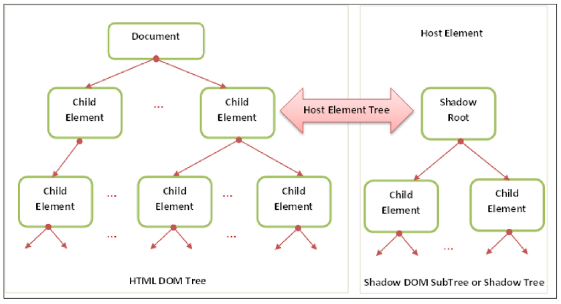
\includegraphics[width=\textwidth,height=\textheight,keepaspectratio]{shaDom.png}
			\caption{DOM und Shadow DOM \cite[S.22]{patel2015learning}}
			\label{img:shaDom}
			\end{figure}\noindent
		\fi
		Die Folge dieser Kapselung ist, dass alles was dem \emph{shadow tree} hinzugefügt wird, nur lokal Einfluss hat. Die Gestaltung von Webelementen im \emph{shadow root} wird dadurch vereinfacht.
		\ac{CSS} Selektoren können dadurch nicht von außerhalb des \emph{shadow roots} auf diesen zugreifen und Selektoren, die innerhalb des \emph{shadow roots} definiert werden, haben keinen Einfluss auf den normalen \ac{DOM}. Genauso verhält es sich mit dem Zugriff auf die \ac{DOM} Elemente des \emph{shadow root}. Sie können nicht von außerhalb angesprochen werden, beispielsweise durch die Funktion \enquote{document.querySelector}, sondern können nur von Funktionen innerhalb des \emph{shadow root} angesprochen werden \cite{Bidelman2016}.
		\begin{listing}
			\begin{JavaScriptcode*}{}
var header = document.createElement('header'); 
var shadowRoot = header.attachShadow({mode: 'open'}); //shadow root an header angefügt
var headline = document.createElement('h1'); 
var headlineText = document.createTextNode('headline');
headline.appendChild(headlineText);
shadowRoot.appendChild(headline); //Elemente als Kinder in shadow root angefügt
			\end{JavaScriptcode*}
				\caption[Erstellung eines Shadow DOM]{JavaScript Programmcode für die Erstellung eines Shadow DOM}
				\label{lst:javShaDom}
		\end{listing}\noindent
		In Listing \ref{lst:javShaDom} ist dargestellt, wie mithilfe von JavaScript ein \emph{Shadow \ac{DOM}} erstellt wird. In Zeile zwei wird zuerst einem bestehendem Element ein \emph{shadow root} hinzugefügt. Daraufhin wird eine Überschrift und deren Text erstellt und zusammengefügt. Zuletzt wird in Zeile sechs die Überschrift in den \emph{Shadow \ac{DOM}} eingefügt.
			\subsubsection{Slots}
			\emph{Shadow \ac{DOM}} kann auch mit anderen \ac{DOM} Elementen erweitert werden. Der Entwickler kann dem Nutzer seines \emph{Web Component} ermöglichen, diesen zu erweitern. Hierfür werden \emph{Slots} verwendet. 
			\begin{listing}
				\begin{HTMLcode*}{}
<ul id='contacts'>
   <li>
      <slot name='title'>Kein Titel</slot> <!-- Slot Element title mit Platzhalter 'Kein Titel' -->
      <slot name='name'> <!-- Slot Element mit Platzhalter -->
         <p>Achtung<p>
         <h1>Kein Name</h1>
      </slot>
   </li>
</ul>
				\end{HTMLcode*}
				\caption[Slot Elemente im Shadow DOM]{HTML Programmcode zur Nutzung von Slot Platzhalter-Elementen im Shadow DOM}
				\label{lst:sloNutShaDom}
			\end{listing}\noindent
			In Listing \ref{lst:sloNutShaDom} ist der \ac{HTML} Programmcode des \emph{Web Component} dargestellt, der im \emph{Shadow \ac{DOM}} später ausgeführt wird. Hier ist die Verwendung des \emph{Slot} Elements interessant. Dieses kann beim Einbinden des \emph{Web Component} später ausgestattet werden. Wird das Platzhalter-Element später nicht befüllt, wird das \emph{Fallback}, also die Ersatzfunktion, der Inhalt innerhalb des Elements, hier beispielsweise \enquote{Kein Titel} genutzt. Die Ersatzfunktion kann auch aus einem eigenen \ac{DOM} Baum bestehen, wie im \emph{Slot} \enquote{name} zu sehen ist \cite{Bidelman2016}. In Listing \ref{lst:sloNutLigDom} werden die, in Listing \ref{lst:sloNutShaDom} erstellten Platzhalter-Elemente, beim Verwenden des \emph{Web Component} in beispielsweise einer Webseite befüllt.
			\begin{listing}[H]
				\begin{HTMLcode*}{}
<span slot='title'>Dr.</span> <!-- Element mit Slot Attribut -->
<span slot='title'>Phil.</span> <!-- Element mit Slot Attribut -->
<span slot='name'>Michael</span> <!-- Element mit Slot Attribut -->
				\end{HTMLcode*}
				\caption[Befüllen der Slot Elemente im DOM]{HTML Programmcode zum Befüllen der Slot Elemente im DOM}
				\label{lst:sloNutLigDom}
			\end{listing}\noindent
		Wie hier in Zeile eins und zwei zu sehen ist, können einzelne Slots auch mit mehreren Elementen befüllt werden. Beim Übersetzen des Programmcodes der Applikation werden alle Elemente, welche die passenden \emph{Slot} Attribute aufweisen in den \ac{DOM} übersetzt. Wenn im \emph{Shadow \ac{DOM}} ein \emph{Slot} Platzhalter ohne ein \enquote{name} Attribut definiert wird, werden alle vom Nutzer innerhalb des \emph{Web Components} erstellten Elemente in den \ac{DOM} geschrieben.
		In Listing \ref{lst:renDom} ist der, von den zwei vorhergehenden Listings,  kombinierte und berechnete Inhalt zu sehen.
		\begin{listing}
			\begin{HTMLcode*}{}
<ul id='contacts'>
	<li>
		<slot name='title'> <!-- Übersetztes Slot Element title -->
			<span>Dr.</span>
			<span>Phil.</span>
		</slot>
		<slot name='name'> <!-- Übersetztes Slot Element name -->
			<span>Michael</span>
		</slot>
	</li>
</ul>
			\end{HTMLcode*}
			\caption{Übersetzter DOM}
			\label{lst:renDom}
		\end{listing}\noindent
		Dies ist der \ac{DOM}, den man beispielsweise in einer Webseite sehen würde. Hier ist gut zu erkennen, wie die \emph{Slot} Elemente des \emph{Shadow \ac{DOM}} mit den später erstellten Elementen befüllt werden. Alle Elemente innerhalb des \emph{Web Component} mit dem Attribut \enquote{slot} werden in diesen übertragen.
		\subsubsection{Shadow DOM Gestaltungsanweisungen}
		Wie auf den vorherigen Seiten erklärt, ist der \emph{shadow tree} vom normalen \ac{DOM} ab gekapselt Dies hat zur Folge, dass \ac{CSS} Gestaltungsanweisungen, definiert im eigenen \emph{Component}, nur Einfluss auf den \emph{shadow tree} des eigenen \emph{Web Component} haben. Es können \ac{CSS} Selektoren verwendet werden, die auch außerhalb des Element bestehen. Trotzdem haben diese nur Einfluss auf die Elemente innerhalb des \emph{Web Component}.  
		 \newline
		Eine Besonderheit der Gestaltungsanweisungen des \emph{Shadow DOM} sind dessen Selektoren. Der \enquote{:host} Selektor definiert den Stil für das Element, in welchem der \emph{shadow tree} bereitgestellt wird, somit für den \emph{Web Component}. Dieser wirkt nur in dem Kontext eines \emph{shadow root}. Dadurch kann der Stil des eigenen \emph{Web Component} verändert werden. Eine Eigenschaft des \enquote{:host} Selektors ist, dass die Seite, die das \emph{Web Component} enthält, stärkeren Einfluss auf diesen Selektor besitzt und somit den Stil überschreiben kann. Damit ermöglicht es den Nutzern eines \emph{Web Component}, diesen von außen nach eigenen Wünschen anzupassen. Darüber hinaus kann der \enquote{:host} Selektor erweitert werden. So können über die Form \enquote{:host(<selector>)} bestimmte Stil Eigenschaften gesetzt werden, die nur Anwendung finden wenn das \emph{Web Component} bestimmte Eigenschaften erfüllt. 
		\begin{listing}
		\begin{HTMLcode*}{}
<style>		
:host(.active) { /* :host Selektor bei Vorhandensein der Klasse active */
   color: green;
}
:host(.blue) { /* :host Selektor bei Vorhandensein der Klasse blue */
   color: blue;
}
</style>
		\end{HTMLcode*}
		\caption[Der :host Selektor]{CSS Gestaltungsanweisungen: Der :host Selektor}
		\label{lst:hosSel}
		\end{listing}\noindent
		In Listing \ref{lst:hosSel} ist dargestellt in welcher Form Einfluss genommen werden kann. So spricht der Selektor in Zeile zwei nur den \emph{Web Component} an, der die Klasse \enquote{active} besitzt. Der Selektor in Zeile fünf spricht nur den \emph{Web Component} an, wenn dieser die Klasse \enquote{blue} besitzt.
		\section{Ein vollständiges Web Component}
		Die in den vorherigen Kapiteln erwähnten Technologien werden nun kombiniert, um beispielhaft ein vollständiges \emph{Web Component} zu erstellen. 		\begin{listing}
			\begin{HTMLcode*}{}
<template>
   <style>
      p {color: red}
   </style>
   <p>Dies ist ein Web Component.</p>
</template>
<script>
class Example extends HTMLElement {
   constructor() {
      super();
      var template = document.currentScript.ownerDocument.querySelector('template');
      var clone = document.importNode(template.content, true);
      this.createShadowRoot().appendChild(clone);
   }
}
customElements.define('example-component', Example);
</script>
			\end{HTMLcode*}
			\caption{Beispiel Web Component}
			\label{lst:beiWebCom}
		\end{listing}\noindent
		In Listing \ref{lst:beiWebCom} ist der \ac{HTML} Programmcode dieser Komponente dargestellt. Hier werden die vorher erwähnten Technologien \emph{Custom Elements}, \emph{Templates} und \emph{Shadow DOM} genutzt. In Zeile eins wird ein \emph{Template} erstellt. Der Inhalt dessen besteht aus den \ac{CSS} Gestaltungsanweisungen und einem Paragraph mit dem Text \enquote{Dies ist ein Web Component.}. Ab Zeile sieben wird der JavaScript Programmcode definiert. Dieser erstellt in Zeile acht die Klasse \enquote{example}, die ein \enquote{HTMLElement} erweitert. Diese besitzt einen Konstruktor. In diesem wird zuerst die \enquote{super} Funktion des erweiterten Element aufgerufen. Danach wird das \emph{Template} Element ausgewählt, dessen Inhalt kopiert und in den neu erstellen \emph{shadow root} eingefügt. In der Zeile 16 wird dann die definierte Komponente zu den \enquote{customElements} unter dem Namen \enquote{example-component} hinzugefügt. Daraufhin kann diese, nachdem die hier erstellte \ac{HTML} Datei importiert wurde, in \ac{HTML} Dokumenten unter dem Bezeichner \enquote{example-component} genutzt werden.
\begin{listing}[H]
	\begin{HTMLcode*}{}
<head>
   <link rel='import' href='comps/example-component.html'>
</head>
<body>
   <p>Normaler Inhalt der Internetseite.</p>
   <example-component></example-component>
</body>
	\end{HTMLcode*}
	\caption{Nutzung des example-component}
	\label{lst:nutExaCom}
\end{listing}\noindent
In Listing \ref{lst:nutExaCom} ist der gesamte \enquote{body} und ein Ausschnitt des \enquote{head} einer \ac{HTML} Datei dargestellt. Diese importiert das in Listing \ref{lst:beiWebCom} erstellte \emph{Web Component} und nutzt es dann unter dem definierten Bezeichner \enquote{example-component}. 
Abbildung \ref{img:beiWebCom} zeigt dann die im Browser angezeigte Ansicht des in Listing \ref{lst:nutExaCom} genutzten \emph{Web Components}. 
\begin{figure}[H]				
	\centering
	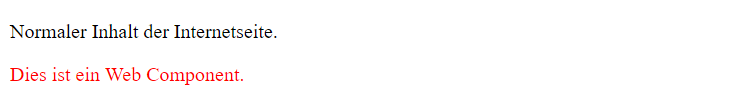
\includegraphics[width=\textwidth,height=\textheight,keepaspectratio]{beiWebCom.png}
	\caption[Ansicht example-component]{Ansicht des Beispiel Web Components Quelle: Bildschirmaufnahme des eigenen, vom Browser übersetzten, Programmcode}
	\label{img:beiWebCom}
\end{figure}\noindent
Hier wird der Text \enquote{Dies ist ein Web Component.} als ein Paragraph angezeigt. Nur dieser Paragraph, also das eigentliche \emph{Web Component} wird in rot dargestellt, da diese Gestaltungsanweisung innerhalb der Komponente gesetzt wurde und somit nur diese betrifft. 
		\section{Webentwicklung mithilfe der Web Components}
		Aktuell werden \emph{Web Components} in der Webentwicklung in geringer Häufigkeit genutzt. Das \emph{Frontend} von modernen Webseiten basiert heutzutage hauptsächlich auf den Technologien \ac{HTML}, \ac{CSS} und JavaScript. Meistens werden darüber hinaus noch verschiedene \emph{Frameworks} verwendet. \enquote{A computer system framework has a layered structure that can incorporate servers, operating systems, client machines, and applications. The framework can provide a set of functions to definde application interfaces, the interrelationships between applications, and internal communications between clients and external to online platforms} \cite[S.15]{stuart2013roadmap}. Ein \emph{Framework} ist somit ein System, das den Entwicklern bestimmte Funktionalitäten zur Verfügung stellt, ohne dass dieser sie selbst programmieren muss. Sie können beispielsweise die Hilfe bei der Interaktion mit dem \ac{DOM} sein, wie das JavaScript \emph{Framework} \enquote{jQuery}, ein \enquote{Slide-Element} bereitstellen wie das \emph{Framework} \enquote{Slider} oder zur Diagrammerstellung genutzt werden wie das \emph{Framework} \enquote{D3}. Hier ergibt sich ein Problem. Wenn in einer Applikation mehrere \emph{Frameworks} und Technologien für verschiedene Funktionen verwendet werden, können diese sich gegenseitig beeinflussen. So können die Gestaltungsanweisungen verschiedener Teile der Webseite sich unbeabsichtigt beeinträchtigen. Auch kann der  JavaScript Programmcode, der eine bestimmte Funktion hat, an einer anderen nicht beabsichtigten, Stelle Einfluss nehmen. An dieser Stelle könnte er eine vollkommen andere Funktion ausüben und Inkonsistenzen hervorrufen. Viele dieser Probleme resultieren daraus, dass verschiedene \emph{Frameworks} für Variablen oder Funktionen die gleiche Benennung nutzen und somit manche Elemente doppelt benannt und damit auch doppelt angesprochen werden. Darüber hinaus können viele Teile der Webseite weder wiederverwendet, noch gut gewartet werden, da sie großen Einfluss aufeinander nehmen und somit sehr ineinander verschachtelt sind.
		Die \emph{Web Components} versuchen diese Probleme durch eine (in Zukunft möglicherweise native) Implementierung verschiedener Techniken anzugehen, die eine Kapselung, eine Wiederverwendung und eine leichtere Wartbarkeit von Programmcode ermöglichen sollen. Nachfolgend wird auf die daraus resultierenden Vor- und Nachteile eingegangen. 			
			\subsection{Native Browser-Unterstützung}
			\label{sec:natBro}
			Aufgrund der Erkenntnisse der Geschichte von \emph{Web Components} in Kapitel \ref{ref:gesVonWebCom} ist eine gewisse Wahrscheinlichkeit gegeben, dass die Technologien der \emph{Web Components} in Zukunft nativ von den verschiedenen Browsern unterstützt werden. Diese Konklusion basiert vor allem auf der Tatsache, dass verschiedene Techniken der \emph{Web Components} schon in manchen Browsern nativ unterstützt werden.
			Sollte dieser Fall eintreffen ergibt sich daraus ein großer Vorteil. Es muss bei der Nutzung nativer, also von den Browsern implementierten Techniken, kein externer Programmcode genutzt werden um bestimmte Funktionen abzudecken. Viele Funktionalitäten können einfach über die Nutzung nativer Methoden abgebildet werden. Deshalb müssen weniger Funktionen selbst geschrieben und weniger, beziehungsweise unter Umständen keine \emph{Frameworks} genutzt werden. Dies verkleinert das Laden vom externen Programmcode. Außerdem ist die Syntax und Funktionsweise bei nativen Funktionen bekannt und eindeutig. Daraus ergeben sich weniger Inkonsistenzen in der Programmierung und eine leichtere Verständlichkeit. Im Gegensatz dazu muss bei vielen \emph{Frameworks} eine jeweils eigene Syntax benutzt werden.
			\subsection{Kapselung}
			Ein Mechanismus zur Datenkapselung wird vom \emph{Shadow DOM} bereitgestellt.
			Dieser ermöglicht, dass der Programmcode des \emph{Web Components} vom Rest der Applikation getrennt werden kann. Dadurch wird ein privater \emph{Scope}, also ein Geltungsbereich der Applikation und dessen Variablen, Methoden und Bezeichnern, genutzt \cite[S.2]{patel2015learning}. Dies hat einige Folgen für das Verhalten einer Applikation. Zuerst ist der \emph{Shadow \ac{DOM}} isoliert. Er kann nicht von außerhalb angesprochen werden. Dies hat den Vorteil, dass die Funktionalität des \emph{Web Component} nicht von außen beeinträchtigt werden kann. Außerdem hat das \ac{CSS} nur Zugriff auf den \ac{DOM} des eigenen Geltungsbereichs; weder von außerhalb noch von innerhalb nach außen des \emph{Shadow \ac{DOM}} können Gestaltungsanweisungen Einfluss nehmen. Ein Vorteil an dieser Eigenschaft ist, dass man atomare, also sehr einfache, \ac{CSS} Bezeichner innerhalb des \emph{Shadow \ac{DOM}} verwenden und dieselben Bezeichner gleichzeitig außerhalb dieses nutzen kann \cite{Bidelman2016}. Atomare Bezeichner haben den großen Vorteil dass sie kurz und prägnant den eigentlichen Nutzen oder Funktion des Elements beschreiben. Darüber hinaus wird die Gestaltung der Erscheinung der Applikation beständiger. Sie erfolgt einzeln für jedes \emph{Web Component} und für den Bereich außerhalb der \emph{Web Components}.
			\subsection{Wiederverwendung}
			Die Theorie der \emph{Web Components} ist die Erstellung von verschiedenen Komponenten, die wiederverwendet werden können. Dies hat zum einen den großen Vorteil, dass es eine Interoperabilität zwischen \emph{Frameworks} ermöglicht \cite[S.2]{patel2015learning}. Dadurch ist man nicht an ein bestimmtes \emph{Framework} gebunden und kann auch mit Elementen außerhalb dieses Ökosystems interagieren und Komponenten wiederverwenden. Zum anderen können die \emph{Web Components} aufgrund ihrer Definitionsart an theoretisch allen Stellen einer Anwendung wiederverwendet werden, was eine Arbeitserleichterung und auch Verminderung des Programmcodes hervorruft. 
			\subsection{Wartbarkeit}
			Die Wartbarkeit von Web-Applikationen wird erleichtert, da die \emph{Web Components} in \emph{Templates} organisiert sind \cite[S.2]{patel2015learning}. Das sorgt dafür, dass der Programmcode einzelner Komponenten separat gespeichert und somit leichter wiedergefunden und geändert werden kann. Insbesondere bei großen Projekten führt dies zu einer großen Arbeitserleichterung.
			\subsection{Browser-Unterstützung}
			\label{sec:broUnt}
			Auch wenn \emph{Web Components} sehr viele Vorteile aufweisen, ist es ein Problem wenn die Techniken (noch) nicht in allen Browsern unterstützt werden oder unterschiedlich implementiert sind. Wie in Kapitel \ref{ref:gesVonWebCom} dargelegt, werden einige der Techniken noch nicht von allen Browsern unterstützt oder unterscheiden sich in deren Umsetzung. Dies kann zu Inkonsistenzen oder dem nicht Funktionieren einer Applikation führen. Durch Verwendung von  \emph{Polyfills} kann man dies jedoch umgehen. Das sind in diesem Zusammenhang Programmcodes, welche die Funktionen oder Teile einer Technologie, die nativ noch nicht von einem Browser unterstützt wird, nachstellen. Sie können dann verwendet werden um Nutzern aller Browser den Gebrauch der Technologien zu ermöglichen \cite[S.4]{satrom2014building}. Das \enquote{webcomponents.js} ist ein Set von \emph{Polyfills} und ermöglicht den Nutzern die Verwendung von \emph{Web Components} in allen modernen Browsern \cite{webComJs}.
	\section{Adaptivität der Web Components?}
	Die Technik und die Vor- und Nachteile von \emph{Web Components} allgemein wurden in den vorhergehenden Kapiteln evaluiert. Daraufhin stellt sich nun die Frage, inwiefern die \emph{Web Components} zur Adaptivität geeignet sind. Um eine Komponente adaptiv zu gestalten, muss es möglich sein auf den Aufbau, das Aussehen und unter Umständen den Inhalt dieser Einfluss nehmen zu können.
	\newline
	Den Aufbau und das Aussehen adaptiv anzupassen könnten die \ac{CSS} Gestaltungsanweisungen innerhalb der \emph{Web Components} ermöglichen. Hier könnten je nach Nutzer andere Gestaltungsanweisungen erfolgen, um die Komponente an den Nutzer anzupassen. Um Einfluss auf den Inhalt nehmen zu können, könnten Methoden innerhalb der Komponente definiert werden, die Inhalt, anhand den Präferenzen des Nutzers, hinzufügen, weglassen oder ändern. Durch den gekapselten Zustand könnten sich bei richtiger Anwendung nur die \emph{Web Components} an den Nutzer adaptiv anpassen und keine anderen Teile der Webseite ungewollt verändern. Dies würde auch ermöglichen jedes einzelne \emph{Web Component} unabhängig zu verändern. Da unter Umständen jedes einzelne \emph{Web Component} anderweitig angepasst werden müsste um die Präferenzen der Nutzer zu erfüllen ist dies eine wichtige Eigenschaft. Um jedoch diese Anpassung innerhalb der \emph{Web Components} durchzuführen muss auch auf innerhalb der Komponenten zugegriffen werden können. Dazu können HTML-Attribute genutzt werden. Diese würden von \enquote{außen} dem \emph{Web Component} hinzugefügt werden und dann innerhalb dieses verwendet werden um bestimmte Anpassungen durchzuführen. Falls alle diese Techniken korrekt genutzt werden und sich nicht gegenseitig negativ beeinflussen, kann es möglich sein \emph{Web Components} zur Adaptivität zu erweitern.
\chapter{Polymer}
Die \enquote{Polymer} Bibliothek bietet eine Möglichkeit \emph{Web Components} zu nutzen. Sie stellt eine Sammlung von Funktionen bereit um \emph{custom elements} zu erstellen und bietet darüber hinaus verschiedene nützliche Funktionen an. Die mithilfe dieser Bibliothek erstellten Elemente sollen letztendlich wie normale \ac{DOM} Bestandteile funktionieren \cite{polymerFeaOve}.
	\section{Polymer Technologie} Die verwendeten Technologien der Bibliothek um \emph{Web Components} zu erstellen ähneln den der \emph{Web Components} oder es werden direkt die Technologien der \emph{Web Components} genutzt. Im Folgenden wird die Technik der Version 1.0 erläutert.
		\subsection{Ein Element registrieren}
		Ähnlich der \emph{Web Components} Technologie, muss mithilfe der \enquote{Polymer} Bibliothek ein vom Entwickler neu erstelltes \enquote{Custom Element} zuerst registriert werden. 
		\begin{listing}
		\begin{JavaScriptcode*}{}
MyElement = Polymer({
	is: 'my-element'
});
// Instanziierung mit createElement
var elem = document.createElement('my-element');
// Instanziierung über Konstruktor
var elem2 = new MyElement();
		\end{JavaScriptcode*}
		\caption[Polymer custom element Registrierung]{JavaScript Programmcode der Polymer custom element Registrierung}
		\label{lst:polCusEle}
		\end{listing}\noindent
Die \enquote{Polymer} Funktion erstellt einen Prototypen eines Elements, registriert diesen im Browser und gibt einen Konstruktor zurück, der genutzt werden kann um Instanzen des Elements zu erstellen. Wie in Listing \ref{lst:polCusEle} in Zeile zwei zu sehen, spezifiziert das \enquote{is} Argument der Funktion den Namen der \ac{HTML} Kennzeichnung (\emph{tag}). In Zeile fünf und sieben sind die beiden Möglichkeiten dargestellt ein Element zu registrieren, also eine Instanz zu erstellen. Einmal über die \enquote{createElement} Funktion oder über den \enquote{new} Operator. In der \enquote{Polymer} Funktion kann das Argument \enquote{extends} hinzugefügt werden. Dieses kann mit einem Wert befüllt werden, der einem Standard \ac{HTML} Element Bezeichner entspricht, beispielsweise \enquote{input}. Dadurch kann dieses Standard \ac{HTML} Element erweitert werden. Bei der Instanziierung über den Konstruktor wird dann genauso wie in Listing \ref{lst:polCusEle} verfahren, bei der Instanziierung durch \enquote{createElement} muss als erstes Argument der Funktion zusätzlich das zu erweiternde Element und als zweites Argument der \enquote{is} Wert des neu erstellten \enquote{Custom Element} übergeben werden, beispielsweise \enquote{var elem = document.createElement('input', 'my-input');} \cite{polyReg}.
\subsection{Laufzeit der Elemente}
\label{sec:polLau}
Um auf die Laufzeit und die Reaktion der Elemente auf deren Zustände im Lebenszyklus zu reagieren stellt \enquote{Polymer} verschiedene \emph{Callback} bereit. Diese werden vom Element selbst ausgeführt, wenn bestimmte Zustände vorliegen. Die \enquote{ready} Funktion wird beispielsweise ausgeführt, wenn der gesamte lokale \ac{DOM} des Elements initialisiert und die Eigenschaftswerte gesetzt wurden. Ein weiteres Beispiel ist die \enquote{attached} Funktion, sie wird aufgerufen wenn das Element an das \enquote{document} hinzugefügt wird. Sie wird in jedem Fall nicht ausgeführt, bevor die \enquote{ready} Rückruffunktion ausgeführt wurde \cite{polyReg}.
\subsection{Eigenschaften der Elemente}
Der Prototyp kann mit Eigenschaften versehen werden. Hierfür wird das \enquote{properties} Objekt genutzt. Es können beliebig viele Eigenschaften des Elements definiert und zu jeder Eigenschaft verschiedene Schlüssel hinzugefügt werden. Der \enquote{type} Schlüssel definiert beispielsweise den Typ des Attributs, in Listing \ref{lst:polProp} ist die Eigenschaft \enquote{user} beispielsweise vom Typ \enquote{String} und die Eigenschaft \enquote{isHappy} vom Typ \enquote{Boolean}.
\begin{listing}[H]
	\begin{JavaScriptcode*}{}
Polymer({
   is: 'my-element', //Bezeichner des Elements
   properties: {  //Eigenschaften des Elements
      user: String, //Eigenschaft mit Datentyp
      isHappy: Boolean,
      count: {
         type: Array,
         value: function() { return {}; }
      }
   }
});
	\end{JavaScriptcode*}
	\caption[Polymer properties Objekt]{JavaScript Programmcode des Polymer properties Objekt}
	\label{lst:polProp}
\end{listing}\noindent
Als weiteres Beispiel definiert der \enquote{value} Schlüssel den Standardwert der Eigenschaft, bei der Eigenschaft \enquote{count} die in der Funktion erstellte leere Datengruppe \cite{polyProp}.
\subsection{Methoden der Elemente}
Um den späteren Instanzen Methoden zur Verfügung zu stellen, können diese dem Prototyp des Elements hinzugefügt werden.
\begin{listing}[H]
	\begin{JavaScriptcode*}{}
Polymer({
   is: 'my-element',
   speak: function(){  //Methode des Elements
	   console.log('speak');
   }
});
//Nachdem das Element instanziiert ist, kann die Methode aufgerufen werden.
var elem = document.querySelector('my-element');
elem.speak();
	\end{JavaScriptcode*}
	\caption[Polymer Instanz-Methoden]{JavaScript Programmcode der Polymer Instanz-Methoden}
	\label{lst:polMeth}
\end{listing}\noindent
In Listing \ref{lst:polMeth} wird dem Prototyp die Methode \enquote{speak} zur Verfügung gestellt. In Zeile neun wird dann die Methode von einer Instanz aufgerufen. Zudem stehen viele verschiedene Methoden standardmäßig jedem Prototyp zur Verfügung. Diese können für verschiedene Zwecke genutzt werden \cite{polyInstMeth}.
\subsection{Polymer DOM}
Polymer unterstützt verschiedene \ac{DOM} Implementierungen. Wird vom genutzten Browser \emph{Shadow DOM}, die Technologie aus dem Bereich der \emph{Web Components} unterstützt, kann diese verwendet werden. Unterstützt der Browser dies nicht, wird eine angepasste Implementierung in \enquote{Polymer} genutzt, der \emph{shady DOM}. Insgesamt sind beide Möglichkeiten in \enquote{Polymer} dem lokalen \ac{DOM} zugeordnet und werden im weiteren so genannt \cite{polLocDom}.
\begin{listing}
	\begin{HTMLcode*}{}
<dom-module id='my-element'> <!-- Wird zu lokalem DOM übersetzt -->
   <template>I am my-element!</template>  <!-- Template Inhalt des Elements -->
   <script>  // Skript des Elements
      Polymer({
      is: 'my-element'
      });
   </script>
</dom-module>
	\end{HTMLcode*}
	\caption{Polymer dom-module}
	\label{lst:polLocDom}
\end{listing}\noindent
In Listing \ref{lst:polLocDom} ist der Programmcode zur Erstellung eines lokalen \ac{DOM} von \enquote{Polymer} dargestellt. Das Element zur Erstellung dieses wird \enquote{dom-module} genannt. Das Element muss im \enquote{id} Attribut den gleichen Wert enthalten wie der Prototyp im \enquote{is} Argument, um eine Zuordnung zu ermöglichen. Es enthält ein \enquote{template} Element in Zeile zwei, dessen Inhalt wird dann in den lokalen \ac{DOM} der Instanz des Prototyps geschrieben. \newline
\enquote{Polymer} Elemente können durch Gestaltungsanweisungen ergänzt werden. Diese sollten, wie standardmäßig bei der Verwendung von \ac{CSS}, innerhalb \enquote{<style>} und darüber hinaus innerhalb des \enquote{<template>} Tags gesetzt werden.
\iffalse
	\newline
	!::content!
\fi
\newline
Kongruent zum \emph{Shadow DOM}, ermöglicht der \emph{shady DOM}, eine Kapselung der Stil-Eigenschaften. Dadurch haben Gestaltungsanweisungen innerhalb des \enquote{Polymer} Elements keinen Einfluss auf außerhalb und umgekehrt. Um dem Nutzer eines \enquote{Polymer} \emph{Web Component} jedoch zu ermöglichen Einfluss auf den Stil dessen zu nehmen, können benutzerdefinierte \ac{CSS} Eigenschaften genutzt werden \cite{polStyLocDom}.
\begin{listing}
	\begin{HTMLcode*}{}
<style>
.title {
	color: var(--my-element-title-color); /* Benutzerdefinierte Eigenschaft */
}
.smalltext {
	color: var(--my-element-smalltext-color, blue); /* Benutzerdefinierte Eigenschaft mit Standardwert */
}
</style>
	\end{HTMLcode*}
	\caption[Benutzerdefinierte CSS Eigenschaften]{Benutzerdefinierte CSS Eigenschaften zur Polymer Web Component Erstellung}
	\label{lst:benCss}
\end{listing}\noindent
Diese werden in der in Listing \ref{lst:benCss} dargestellten Form, im Bereich der Stil-Eigenschaften, bei der Erstellung eines \enquote{Polymer} Elements definiert. Wie in Zeile sechs zu sehen ist kann auch, falls der Nutzer der Eigenschaft keinen Wert zuweist ein Standard Wert gesetzt werden. Hier ist der Standardwert \enquote{blue}. An einer Stelle oberhalb des \ac{DOM} kann dann die \ac{CSS} Eigenschaft \enquote{--my-element-title-color} vom Nutzer des Elements mit einem Wert belegt werden. Dadurch wird ab dann jedes Element das mit dieser benutzerdefinierten Eigenschaft belegt ist, mit dem vom Nutzer gesetzten Wert ausgezeichnet. Beispielsweise kann der \enquote{:host} Selektor mit der Eigenschaft \enquote{--my-element-title-color: green} ausgezeichnet werden. Dadurch werden alle Elemente innerhalb des \emph{shadow root}, mit der benutzerdefinierten Eigenschaft \enquote{--my-element-title-color} auf den Wert \enquote{green} gesetzt.
\chapter{Das AWC Framework}	
Das \ac{AWC Framework} ist eine weitere Möglichkeit mit \emph{Web Components} zu arbeiten. Es wurde von der \enquote{REMEX} Forschungsgruppe entwickelt. Das JavaScript \emph{Framework} wird auch mit der Bezeichnung \enquote{Darwin.js} beschrieben. Es soll die Implementierung von adaptiven Benutzeroberflächen ermöglichen, basierend auf der Technik der \emph{Web Components}. Die Oberflächen richten sich somit nach den Bedürfnissen und der Zusammenstellung der Präferenzen eines Nutzers, um die Zugänglichkeit, Gebrauchstauglichkeit und das Nutzungserlebnis zu verbessern \cite{darwin}. Im Folgenden wird die verwendete Technik des \ac{AWC Framework} auf Basis des auf \enquote{GitHub} vorhandenen Programmcodes erläutert \cite{gitHubAwc}. 
\section{Darwin.js Technologie}
Um ein neues adaptives \emph{Web Component} zu erstellen wird die Klasse \enquote{Component} und von dieser der Konstruktor genutzt. Diesem können vier Parameter übergeben werden. Sie setzen sich aus \enquote{\_htmlTag}, \enquote{\_baseClass}, \enquote{\_data} und \enquote{\_options} zusammen. Zu Beginn nutzt der Konstruktor die Methode \enquote{testBrowserSupport} um abzufragen, ob die Technologien der \emph{Web Components} vom Browser unterstützt werden. Ist dies nicht der Fall tritt eine Fehlermeldung auf. Danach wird mit den übergebenen Parametern weitergearbeitet.
	\subsection{Registrierung eines Elements}
	 Der Parameter \enquote{\_htmlTag} definiert den Bezeichner unter dem das neue Element registriert wird, während der Parameter \enquote{\_baseClass} definiert, welches \ac{HTML} Element als Basis genutzt wird und erweitert wird. Hier kann zum Beispiel das \enquote{Button} Element definiert werden. Das Elternelement aller \ac{HTML} Elemente ist das \enquote{HTMLElement}, dieses kann auch expandiert werden wenn kein bestimmtes, schon bestehendes, Element erweitert werden soll. In Listing \ref{lst:awcErs} ist der Programmcode dargestellt, der ein neues Element erstellt. Hier wird das Element unter dem Bezeichner \enquote{awc-image} und als Erweiterung des \enquote{HTMLElement} registriert.
	 \begin{listing}
	 	\begin{JavaScriptcode*}{}
new Component('awc-image', HTMLElement,
   // Modell des Elements:
   {
      'contrast': 'normal',
      'size': 'normal',
      'reading_direction': 'ltr'
   },
   // Verhalten des Elements:
   {
      onAdaptiveChange: function() {
      console.log('onAdaptiveChange');
      console.log(this);
   }
});
	 	\end{JavaScriptcode*}
	 	\caption[Web Component basierend auf Darwin.js]{JavaScript Programmcode zum Erstellen eines Web Components basierend auf Darwin.js}
	 	\label{lst:awcErs}  
	\end{listing}\noindent
	\subsection{Eigenschaften der Elemente}
	Dem \enquote{\_data} Parameter werden die initialen Modelldaten übergeben. Hier können die eigentlichen Präferenzen oder Einstellungen der späteren Nutzer mit initialen Werten gespeichert werden. Es können beliebig viele Präferenzen-Wert Paare übergeben werden. In Listing \ref{lst:awcErs} werden beispielsweise die Präferenzen \enquote{contrast}, \enquote{size} und \enquote{reading\_direction} gesetzt.
	\subsection{Methoden der Elemente}
	Dem \enquote{\_options} Parameter können optional Methoden übergeben werden. Dadurch erhält das \emph{Web Component} initial diese Funktionalität und kann zur Laufzeit verwendet werden. Bei der Erstellung des \enquote{awc-image} in Listing \ref{lst:awcErs} wird beispielsweise die Methode \enquote{onAdaptiveChange} übergeben. Diese wird somit dem \emph{Web Component} zugeordnet.
	\subsection{Bilden eines Elements}
	Um das Element letztendlich zu bilden werden verschiedene Schritte im Konstruktor der \enquote{Component} Klasse durchgeführt. Zu Beginn muss ein \emph{shadow root} geschaffen werden, das wird in Listing \ref{lst:shaRoo} dargestellt.
	\begin{listing}
		\begin{JavaScriptcode*}{}
this.root = this.attachShadow({
   mode: 'open' //Offener shadow root
});
		\end{JavaScriptcode*}
		\caption[Erstellung des shadow roots]{JavaScript Programmcode zum Erstellen des shadow roots}
		\label{lst:shaRoo}  
	\end{listing}\noindent
	Daraufhin wird der zu importierende \emph{Link}, passend zum \enquote{\_htmlTag}, gewählt. Von diesem \emph{Link} wird das \emph{Template} Element gespeichert. Daraufhin wir die Funktion \enquote{\_buildHtml} mit dem Parameter \enquote{data} aufgerufen. Diese ist in Listing \ref{lst:bilDar} dargestellt.
		\begin{listing}
		\begin{JavaScriptcode*}{}
_buildHtml(data) {
   this.root.innerHTML = ''; //leerer shadow root
   let instance = this.template.content.cloneNode(true); //Kopieren des Inhalts
   let div = document.createElement('div'); 
   div.appendChild(instance); //Inhalt wird als Kind an das div angehängt
   let handlebar = window.Handlebars.compile(div.innerHTML); //Inhalt des div wird mit Handlebars kompiliert
   let buildHtml = handlebar(data); //Kompilierter Code wird mit data Werten ausgeführt
   this.root.innerHTML = buildHtml; //shadow root wird befüllt
}
		\end{JavaScriptcode*}
		\caption[Bilden des Web Components]{JavaScript Programmcode zum Bilden eines Web Components basierend auf Darwin.js}
		\label{lst:bilDar}
		\end{listing}\noindent
	Hier wird in Zeile eins der Inhalt des \emph{shadow root} geleert. Daraufhin wird der Datenknoten des Inhalts des \emph{Templates} kopiert. Dieser wird dann als Kind eines neu erstellten \emph{div} Elements in Zeile fünf hinzugefügt. Daraufhin wird der Inhalt dieses \emph{divs} mithilfe des \enquote{Handlebar} \emph{Frameworks} kompiliert. \enquote{Handlebar} ermöglicht semantische \emph{Templates} zu erstellen. In diesen \emph{Templates} können Ausdrücke innerhalb vier geschweifter Klammern gesetzt werden, beispielsweise wie: \enquote{\{\{Inhalt\}\}}. Diese funktionieren als Platzhalter und werden beim Kompilieren durch die gesetzten Werte ersetzt \cite{handlebars}. In Zeile sieben wird daraufhin der kompilierte Inhalt mit dem \enquote{data} Objekt als Parameter ausgeführt. Dadurch werden alle Platzhalter des \emph{Templates} durch die richtigen Werte ersetzt. Zuletzt wird der Inhalt des \emph{shadow root} mit dem kompilierten Inhalt, also dem Programmcode des \emph{Web Component}, befüllt.
	\subsection{Adaptivität der Elemente}
	\label{sec:adaDerEle}
	Die Adaptivität der Elemente wird über verschiedene Aktualisierungsmethoden ermöglicht. Diese werden in der Klasse \enquote{Components} definiert. Die Methode \enquote{update} ändert die Eigenschaften aller \emph{Web Components} einer bestimmten Art, zum Beispiel alle \enquote{awc-image} Elemente. Sie erwartet zwei Parameter, den \enquote{htmlTag} der zu verändernden Elemente und \enquote{data}, die neuen Werte der Elemente. Zu Beginn wird die Methode \enquote{\_hasAdaptiveWebComps} genutzt um abzufragen, ob der Browser die Funktionalitäten, die zur Adaptivität benötigt werden, besitzt. Wenn dies zutrifft werden alle Elemente gesammelt, die den bestimmten \enquote{htmlTag} besitzen. Daraufhin wird an jedes dieser Elemente ein Ereignis mit der Bezeichnung \enquote{adaptiveUpdate} gesendet, dem das \enquote{data} Objekt angehängt wird.
	In der Klasse \enquote{Component} wird über die Registrierung eines \enquote{EventListener} für jedes \emph{Web Component} dieses Ereignis empfangen. Daraufhin wird die Methode \enquote{\_adaptiveChangeCallback} aufgerufen. Diese führt zu Beginn die Methode \enquote{\_pipeCallback} mit dem Parameter \enquote{onAdaptiveChange} aus, dadurch werden etwaige \emph{Callback} Funktionen des Elements mit dem Wert dieses Parameters ausgeführt. Danach fügt sie die neuen \enquote{data} Werte mit den vorhandenen des \emph{Web Component} zusammen und bildet das Element mit den Werten neu.
	\newline
	Die Methode \enquote{updateAll} ändert die Eigenschaften aller auf der Seite vorhandenen \emph{Web Components}. Als Parameter erwartet sie das \enquote{data} Objekt mit den neuen Werten für die Eigenschaften der Elemente. Wird sie aufgerufen prüft sie zu Beginn auch über die Methode \enquote{\_hasAdaptiveWebComps}, ob der Browser die Funktionalitäten, die zur Adaptivität benötigt werden, besitzt. Daraufhin werden alle \emph{Web Components} der Anwendung gesammelt und wiederum das Ereignis \enquote{adaptiveUpdate} an jedes dieser Elemente gesendet. Bei diesem Ereignis werden auch die neuen Werte in Form des \enquote{data} Objekts angehängt. Dieses Ereignis wird wie in Kapitel \ref{sec:adaDerEle} von den \emph{Web Components} empfangen und verarbeitet. Letztendlich wird das Element mit den neuen Werten auch wieder neu gebildet und hat sich somit adaptiv angepasst.
	\newline
	Zuletzt muss jedes \emph{Web Component}, beziehungsweise dessen Darstellung, auf diese Anpassung reagieren. Im Werkszustand besitzen diese verschiedene CSS-Klassen. In Listing \ref{lst:temAwcImg} ist der \ac{HTML} Inhalt des \enquote{awc-image} dargestellt.
	\begin{listing}
		\begin{HTMLcode*}{}
<template>
   <img class="contrast_{{ contrast }} reading_direction_{{ reading_direction }} size_{{ size }}" src="/assets/img/carole.png" alt="Carole"> <!-- Element mit CSS Klassen und Handlerbar Platzhaltern -->
</template>
		\end{HTMLcode*}
		\caption[Das awc-image Element]{HTML Programmcode des Templates des awc-image Elements}
		\label{lst:temAwcImg}
	\end{listing}\noindent
	In diesem besitzt das \emph{img} Element einige CSS Klassen. Klassen die zur Bereitstellung der Adaptivität genutzt werden, starten mit dem Namen der Präferenz und einem Unterstrich, beispielsweise \enquote{contrast\_} und sind gefolgt von einem \enquote{Handlebar} Platzhalter, dessen Inhalt wiederum der Name der Präferenz ist, hier \enquote{\{\{contrast\}\}}. Jede Neubildung oder Änderung des Elements ändert mithilfe des \enquote{Handlebar} \emph{Frameworks} die CSS-Klassen des Elements. Je nach gesetzter CSS Klasse wird das Element dann anders dargestellt. 
	\begin{listing}
		\begin{CSScode*}{}
.contrast_, .contrast_normal { /* Standardkontrastwert */
   -webkit-filter: none;
   filter: none;
   background: #fff;
}
.contrast_high { /* Erhöhter Kontrastwert */
   -webkit-filter: grayscale(100%) contrast(130%);
   filter: grayscale(100%) contrast(130%);
   background: #000;
}
		\end{CSScode*}
		\caption[CSS Programmcode awc-image]{Ausschnitt der CSS Gestaltungsanweisungen des Templates des awc-image}
		\label{lst:cssAwcIma}
	\end{listing}\noindent
	In Listing \ref{lst:cssAwcIma} sind ein Ausschnitt der Darstellungseigenschaften des \emph{Web Component} gezeigt. Sie bestimmen inwiefern sich die Darstellung ändert. So wird in der Standarddarstellung des Kontrastwerts (\enquote{contrast\_} und \enquote{contrast\_normal}) ein weißer Hintergrund und kein CSS-Filter genutzt. Ist jedoch die \ac{CSS} Klasse \enquote{contrast\_high} gesetzt, ist die Präferenz des Nutzers ein erhöhter Kontrastwert. Dann wird ein \ac{CSS} Filter \enquote{grayscale(100\%) contrast(130\%)} und eine schwarze Hintergrundfarbe genutzt. Dies erhöht den Kontrast der Darstellung des Elements.
\section{Beispiel eines AWC Web Component}
	Mithilfe des AWC \emph{Frameworks} wird im Folgenden ein \emph{Web Component} erstellt. Es wird unter dem Namen \enquote{awc-input} registriert und hat die Funktion einen Benutzer nach einer Frage zu einem von ihm zu wählenden Thema zu befragen.
	\begin{listing}
	\begin{HTMLcode*}{}
<div class="contrast_{{ contrast }} reading_direction_{{ reading_direction }} size_{{ size }}">
	<p>Hallo{{ name }}, bitte wähle dein Thema:</p>  <input name="topic" type="text">
	<p>Deine Frage ist:</p> <textarea name="question" cols="40" rows="5"></textarea>
	<button type="button">Absenden</button>
</div>
	\end{HTMLcode*}
	\caption[Das awc-input Element]{HTML Programmcode des awc-input Element}
	\label{lst:awcInp}
\end{listing}\noindent
	In Listing \ref{lst:awcInp} ist ein Ausschnitt des Elements, der HTML Programmcode des Elements, dargestellt. Hier wird in Zeile zwei ein \enquote{input} Feld erstellt, das den Nutzer nach dem gewünschten Thema fragt, in Zeile drei wird ein \enquote{textarea} Feld erstellt, das den Nutzer nach seiner Frage bittet. Zuletzt wird in Zeile vier ein \enquote{button} erstellt, der, bei Anbindung an das \emph{Backend}, die Frage abschickt. In Listing \ref{lst:awcInpJavScr} ist der JavaScript Programmcode des Elements dargestellt.
	\begin{listing}
		\begin{JavaScriptcode*}{}
new Component('awc-input', HTMLElement,
	// Modell:
	{
		'contrast': 'normal',
		'reading_direction': 'ltr',
		'size': 'normal'
	},
	// Verhalten:
	{
		onAdaptiveChange: function() {
			console.log('onAdaptiveChange');
			console.log(this);
		}
	});
		\end{JavaScriptcode*}
		\caption[JavaScript Programmcode awc-input]{JavaScript Programmcode des awc-input}
		\label{lst:awcInpJavScr}
	\end{listing}\noindent
	Hier wird das Element unter dem Namen \enquote{awc-input} registriert und seine standardmäßigen Werte der Präferenzen gesetzt. Die Präferenzen des Elements können dann über das AWC \emph{Framework} verändert werden, dabei werden seine Klassen geändert. Daraufhin ändert das Element sein Aussehen aufgrund dieser Klassen, anhand von Gestaltungsanweisungen. In Abbildung \ref{img:awcInput} ist das Elemente dargestellt.
	\begin{figure}[H]				
		\centering
		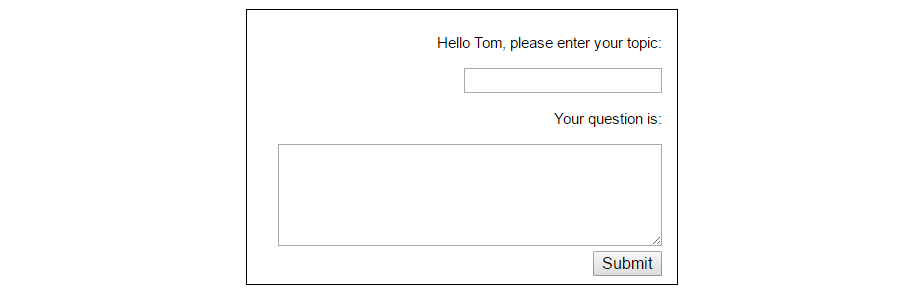
\includegraphics[width=\textwidth,height=\textheight,keepaspectratio]{awcInput.png}
		\caption[Ansicht awc-input]{Ansicht des awc-input Elements Quelle: Bildschirmaufnahme des eigenen, vom Browser übersetzten, Programmcode}
		\label{img:awcInput}
	\end{figure}\noindent
	Hier wird es von einem Nutzer aufgerufen, der eine normale Schriftgröße, einen normalen Kontrastwert und eine Leserichtung von rechts nach links in seinen Präferenzen festgelegt hat.
\chapter{Adaptivität von bestehenden Web Components}
\label{sec:adaVonBesWebCom}
	In den folgenden Kapiteln werden bestehende \emph{Web Components} ausgewählt, untersucht und um eine Adaptivität zu ermöglichen, angepasst. Hierfür werden Elemente aus dem Katalog der Internetseite \enquote{customelements.io} gewählt \cite{cusEleIo}. In dieser Ausarbeitung wird nur deutschsprachiger Text beachtet, da eine korrekte Übersetzung sehr vieler möglicher Sprachen schwer durchführbar ist und für eine beispielhafte Konzeption und Programmierung von Adaptivität nicht notwendig ist.
	\section{Iron Data Table}
	Die erste Auswahl fiel auf das Element \enquote{iron-data-table} \cite{saulis}. Dieses \emph{Web Component} stellt Tabellen dar. Die Tabelleninhalte können frei definiert werden.
	\subsection{Konzeption zur Adaptivität}
	\label{sec:konZurAda}
	In der Abbildung \ref{img:datTab} ist das Element, befüllt mit Beispieldaten, dargestellt. Der Aufbau besteht aus der Kopfzeile im oberen Bereich mit den Bezeichnern der Spalten. Darunter ist der eigentliche Inhalt: Für jedes Datenelement eine Zeile mit den Werten des Elements zum Bezeichner der jeweiligen Spalte. Jede Zeile besitzt auf der linken Seite ein Quadrat, das angewählt werden kann und die Funktion besitzt, das Element der jeweiligen Zeile auszuwählen. Das Quadrat der Kopfzeile besitzt die Funktion alle Spalten anzuwählen.
	\begin{figure}[H]		
		\centering
		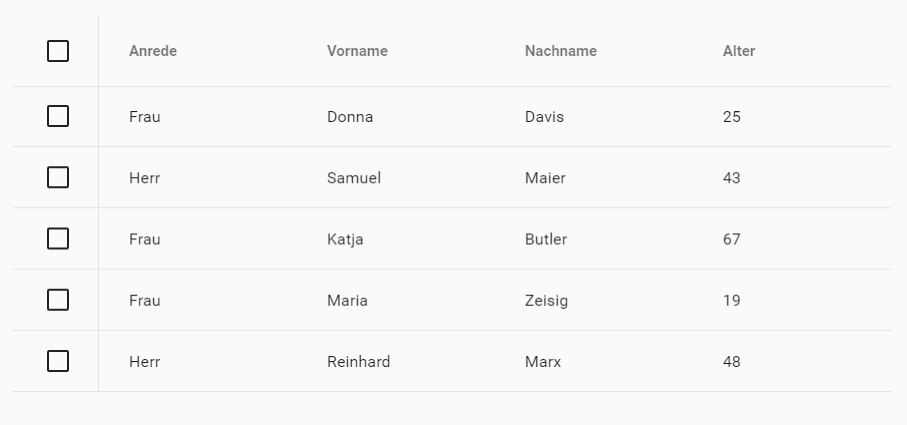
\includegraphics[width=\textwidth,height=\textheight,keepaspectratio]{datTab.png}
		\caption[Iron Data Table]{Iron Data Table Web Component Ansicht \cite{saulis}}
		\label{img:datTab}
	\end{figure}\noindent
	Das Element nutzt Symbole und Texte. Diese sollten sich adaptiv an den Nutzer anpassen. So sollte sich im Bezug auf die Texte Einfluss auf die Schriftgröße, die Schriftart und Text-Alternativen genommen werden. In diesem Element können keine Symbole als Text-Alternativen genutzt werden. Dies liegt daran, dass die Text-Elemente dieser Komponente sich in jeder Tabelle ändern können und somit nicht eindeutig und verlustfrei durch Bilder ersetzt werden können. Im Bezug auf die Symbole sollten Alternativen für diese bereitgestellt werden. Allgemein sollte sich der Kontrast des \emph{Web Components} anpassen und der Aufbau an die Leserichtung des Nutzers anpassen lassen. Die Leserichtung hat einen Einfluss auf die Textelemente, hier werden jedoch nur einzeln stehende Wörter verwendet, die darüber hinaus sich, je nach Inhalten auch verändern. Deshalb lassen sich diese nicht adaptiv anpassen. Jedoch verändert die Leserichtung den Aufbau der Komponente, bisher spiegelt der Aufbau die Relevanz der Spalten wieder, von links nach rechts. Links ist das wichtigste Element, das Quadrat zum Anwählen einer Zeile. Bei einer Leserichtung von rechts nach links wird dieser Aufbau gespiegelt.  
	\subsection{Einrichtung des Iron Data Table}
	Das \emph{Iron Data Table Web Component} ist auf \enquote{GitHub} gespeichert \cite{saulis}. Hier wurde ein \enquote{fork} durchgeführt um am Programmcode dieses Elements weiterarbeiten zu können. Das bedeutet, dass der Stand der eigentlichen Entwicklern kopiert wird und eigene Änderungen im Weiteren darauf aufbauen. Die Abhängigkeiten werden über \enquote{Bower} installiert. \enquote{Bower} ist ein Paketverwaltungsprogramm, welches das Aktualisieren und Installieren von Bibliotheken und \emph{Frameworks} unterstützt. Dabei wird \enquote{Bower} als ein Kommandozeilenprogramm genutzt \cite{bower}. Der \enquote{Iron Data Table} selbst wird aus verschiedenen \emph{Web Components} zusammengesetzt. In der hier verwendeten Zusammenstellung werden die Elemente \enquote{iron-data-table}, \enquote{iron-list}, \enquote{data-table-colum}, \enquote{data-table-row}, \enquote{data-table-checkbox} und \enquote{data-table-cell}  genutzt.  
	\subsection{Umsetzung der Programmierung}
	Im Folgenden wird die konzipierte Adaptivität der Komponenten im Programmcode umgesetzt.
	\subsubsection{Kontrast}
	Um den Kontrast des Elements anzupassen wird die Methode \enquote{\_changeContrast} des \enquote{iron-data-table} Elements genutzt. Diese fragt den Wert des Parameters \enquote{moreContrast} ab, bei einem \enquote{true} Wert wird zu Beginn die Hintergrundfarbe des Hintergrunds auf weiß gesetzt, damit die Elemente sich besser von diesem abheben. Daraufhin werden allen Elementen mit den Bezeichnern \enquote{iron-data-table}, \enquote{data-table-row} und \enquote{data-table-checkbox} die CSS Klasse \enquote{more-contrast} hinzugefügt. Diese werden dann von den einzelnen Komponenten über Gestaltungsanweisungen genutzt. Das umschließende Element \enquote{iron-data-table} wird angewiesen die Schriftfarbe auf schwarz zu setzen um den Kontrast zwischen Text-Elementen und Hintergrund zu erhöhen. Die Komponente \enquote{data-table-row} wird angewiesen einen Rahmen um die Kopfzeile der Tabelle zu erstellen, um eine bessere Abgrenzung dieser vom Rest der Tabelle zu ermöglichen. Auch wird die Farbe des Hintergrunds der Kopfzeile auf weiß gesetzt um den Kontrast zum Text zu erhöhen. Darüber hinaus wird der \enquote{Fokus} Zustand der Zeilen verändert. Dieser wird, vorher dargestellt durch einen blauen Text auf grauem Hintergrund, nun dargestellt durch einen weißen Text auf schwarzem Hintergrund. Dabei wird die blaue Linie unter der Zeile entfernt. Die Komponente \enquote{data-table-checkbox} wird dahingehend verändert, über Gestaltungsanweisungen das Anwählen eines Feldes über einen schwarzen Haken auf weißem Grund statt eines blauen Hakens auf weißem Grund darzustellen.
	\subsubsection{Text-Alternativen}
	In diesem Elemente können Texte wie in Kapitel \ref{sec:konZurAda} dargestellt, nicht durch Symbole ersetzt werden. Jedoch können die vorhandenen Symbole adaptiv durch Texte ersetzt werden. Dies betrifft die Symbole für eine angewählte Zeile, ein Quadrat mit Haken in diesem und die Symbole für eine nicht ausgewählte Zeile, ein Quadrat. Hierfür wird die Methode \enquote{\_changeTextAlternatives} innerhalb des \enquote{iron-data-table} Elements genutzt. Diese fragt zu Beginn den Wert der Eigenschaft \enquote{textAlternatives} ab, ist dieser \enquote{text}, werden alle \enquote{data-table-checkbox} Elemente gesammelt und jedem dieser die CSS Klasse \enquote{text} hinzugefügt und der Inhalt dieses Element durch den Text \enquote{auswählen} ersetzt. Darüber hinaus wird die Methode \enquote{\_changeTextAlternatives} innerhalb des \enquote{data-table-checkbox} Element genutzt. Diese wird von der schon vorhandenen Methode \enquote{\_checkedChanged} aufgerufen. Danach sammelt sie alle \enquote{data-table-checkbox} Elemente und ersetzt den Inhalt dieser durch den Text \enquote{gewählt}, wenn die sie die Klasse \enquote{text} und das Attribut \enquote{checked} enthalten oder durch den Text \enquote{auswählen}, wenn sie nur die Klasse \enquote{text} enthalten und nicht das Attribut \enquote{checked}.
	\subsubsection{Schriftart}
	Die Schriftart sollte sich adaptiv an den Nutzer anpassen. Um dies zu erreichen wird die Methode \enquote{\_changeFontStyle} des \enquote{iron-data-table} Element genutzt. Hier wird der Parameter \enquote{fontStyle} abgefragt. Ist dieser auf den Wert \enquote{serif} gesetzt, wird dem \enquote{iron-data-table} Element die CSS Klasse \enquote{serif} hinzugefügt. Diese wird dann in den Gestaltungsanweisungen genutzt um die Anweisung zur \enquote{font-family} zu ändern.
	\subsubsection{Schriftgröße}
	Auch die Größe der Schrift sollte sich adaptiv an den Nutzer anpassen. Hierfür wird die Methode \enquote{\_changeFontSize} des \enquote{iron-data-table} Elements genutzt. Sie fragt den Wert des Parameters \enquote{fontSize} ab. Dessen Standardwert ist \enquote{m}. Ist der Wert auf \enquote{l} oder \enquote{xl} gesetzt wird die Schriftgröße um zwei oder vier Pixel erhöht. Dies wird ermöglicht durch das Hinzufügen von den CSS Klassen \enquote{l} oder \enquote{xl} zu dem \enquote{iron-data-table} Element. Diese werden dann über Gestaltungsanweisungen des \emph{Web Component} genutzt um die Anweisung zur \enquote{font-size} zu ändern.
	\subsubsection{Leserichtung}
	An die Leserichtung des Nutzers wird sich über die Methode \enquote{\_changeReadingDirection} des \enquote{iron-data-table} Elements angepasst. Sie fragt den Wert des Parameters \enquote{readingDirection} ab. Ist dieser \enquote{rtl}, werden alle \enquote{data-table-row} Elemente gesammelt und jedem dieser die CSS Klasse \enquote{rtl} hinzugefügt. Im den \enquote{data-table-row} Elementen werden diese Klassen in den Gestaltungsanweisungen genutzt, den Wert der \enquote{flex-direction} auf den Wert \enquote{row-reverse} zu setzen um den Aufbau der Zeile zu verändern. Dadurch wird dieser vertikal gespiegelt und das wichtigste Element befindet sich bei einer Leserichtung von rechts nach links auf der rechten Seite.
	\subsection{Beispiel-Ergebnis der Adaptivität}
	In der Abbildung \ref{img:datTabErg} ist das adaptive \enquote{Iron Data Table} Element  dargestellt. Die Abbildung basiert auf dem vorher ausgewählten und daraufhin zur Adaptivität erweiterten Element. 
	\begin{figure}[H]		
		\centering
		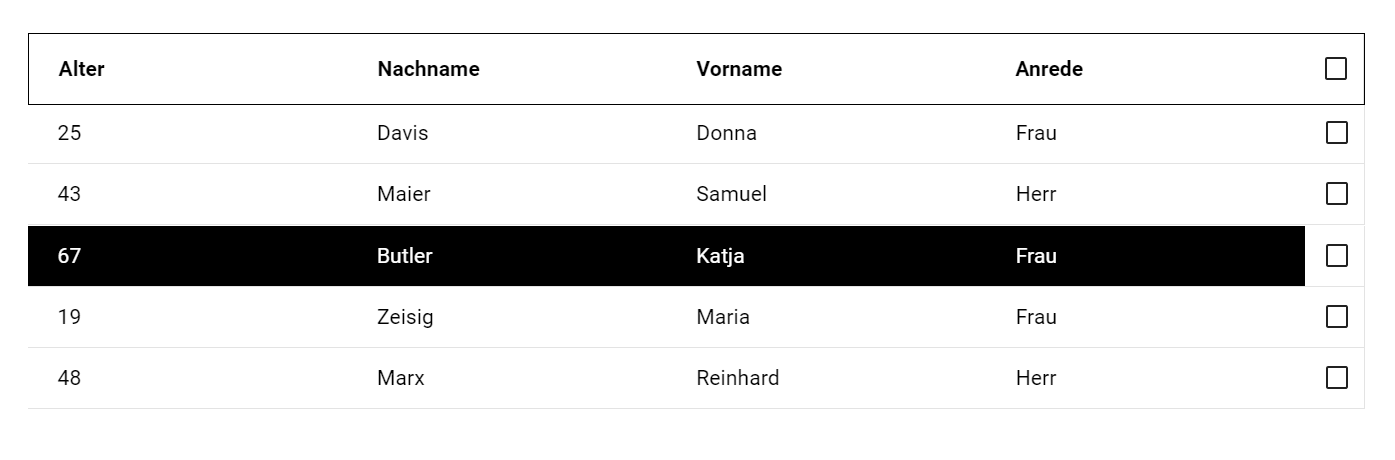
\includegraphics[width=\textwidth,height=\textheight,keepaspectratio]{datTabErg.png}
		\caption[Adaptiver Iron Data Table]{Adaptives Iron Data Table Web Component Ansicht Quelle: Bildschirmaufnahme des eigenen, vom Browser übersetzten, Programmcode}
		\label{img:datTabErg}
	\end{figure}\noindent
	Das Element wurde hier beispielhaft an einen Nutzer angepasst, dessen Präferenzwerte einen erhöhten Kontrast, eine erhöhte Schriftgröße und eine Leserichtung von rechts nach links enthalten. 
	\newpage	
	\section{Paper Date Picker}
	Als nächstes wurde das \enquote{paper-date-picker} Element ausgewählt \cite{datPic}. Es ermöglicht die Anzeige eines Kalenders. Von diesem Kalender kann ein einzelner Tag vom Nutzer ausgewählt werden, dieser wird dann mit erweiterten Informationen angezeigt.
		\subsection{Konzeption zur Adaptivität}
		Das \emph{Web Component} ist in Abbildung \ref{img:datPic} dargestellt.
		Es nutzt Texte und Symbole. Die Adaptivität dieses Elements sollte durch eine mögliche Veränderung des Kontrastes, der Schrift, wenn möglich der Bereitstellung von Text- und Symbol-Alternativen und der Leserichtung und dadurch wiederum der Anordnung der Elemente ermöglicht werden.
		\begin{figure}[H]		
			\centering
			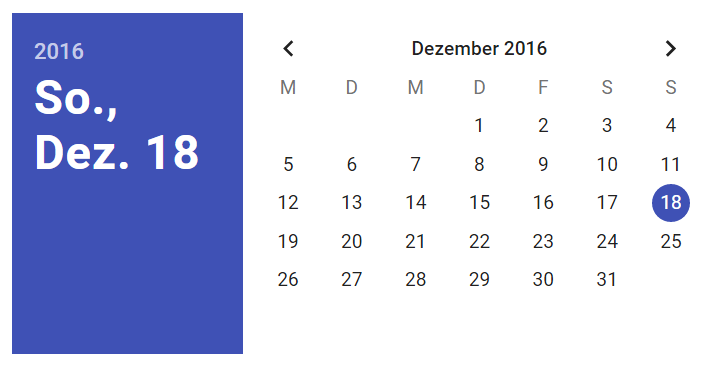
\includegraphics[width=0.7\textwidth,height=\textheight,keepaspectratio]{datPic.png}
			\caption[Paper Date Picker]{Paper Date Picker Web Component Ansicht \cite{papDatPicGit}}
			\label{img:datPic}
		\end{figure}\noindent
		Der Kontrast der Texte, also der Datenelemente, gegenüber dem Hintergrund sollte sich an die Bedürfnisse der Nutzer anpassen. Diese sollten sich hochgradig voneinander unterscheiden lassen können. 
		Es sollten, wenn möglich, Alternativen für Texte oder im Gegensatz dazu, zu Darstellungen, geboten werden. Um Text-Alternativen für Text-Elemente zu ermöglichen muss es möglich sein diese zu ersetzen ohne ein Verlust an Informationen zu erleiden. Die Text-Komponenten dieses Elements bestehen aus Bezeichnungen für Tage, Monate, Jahre und Zahlen. Es ist nicht möglich, diese durch eindeutige Symbole zu ersetzen. Deshalb können in diesem \emph{Web Component} keine Text-Alternativen angeboten werden. Es werden jedoch auch Symbole in diesem \emph{Web Component} genutzt. Um zwischen den Monaten des Datums-Wählers zu wechseln werden Vergleichszeichen genutzt. Um zu einem Monat vorher zu wechseln wird das Kleiner-als-Zeichen und um zu einem Monat später zu wechseln wird das Größer-als-Zeichen genutzt. Jeweils bei einem Klick auf eines dieser Symbole wird dessen Funktionalität ausgeführt. Eine Alternative für diese Symbole kann durch verschiedene Sätze bereitgestellt werden. So kann das Symbol für den vorherigen Monat durch den Ausdruck \enquote{voriger Monat} und für den nächsten Monat durch den Ausdruck \enquote{nächster Monat} ersetzt werden.
		Auf die Schrift der Texte sollte Einfluss genommen werden können. So sollte die Schriftart und insbesondere die Schriftgröße anpassbar sein. Die Schriftart sollte zwischen einer serifen und einer serifenlosen Art wechseln, die Größe sollte sich zwischen der Standardgröße, einer großen und einer sehr großen Schriftgröße wechseln lassen. Hiervon sind Datenelemente und die Bezeichner des Kalenders betroffen. Auch der Text des derzeitig ausgewählten Datums sollte sich anpassen können.
		Um sich an die Leserichtung des Nutzers anzupassen, sollte Einfluss auf die Anordnung der Texte und auch Elemente genommen werden. Der Standardzustand der Komponente ist die Leserichtung von links nach rechts, hier wird das ausgewählte Datum auf der linken Seite und der Kalender auf der rechten Seite dargestellt. Auch werden die Wochentage des Kalenders von links nach rechts gelesen. Diese Elemente sollten sich bei einer Leserichtung von rechts nach links verschieben lassen.  
		\subsection{Einrichtung des Paper Date Picker Web Component}
		Das \emph{Paper Date Picker Web Component} ist auf \enquote{GitHub} gespeichert \cite{papDatPicGit}. Es wurde wiederum ein \enquote{fork} durchgeführt um an diesem weiterarbeiten zu können und es zu erweitern. Für die Abhängigkeiten des Elements wurde wieder \enquote{Bower} genutzt. Das \enquote{Paper Date Picker} Element wird selbst aus verschiedenen \emph{Web Components} zusammengesetzt. In der hier verwendeten Zusammenstellung werden insgesamt die Elemente \enquote{paper-date-picker}, \enquote{paper-calendar}, \enquote{paper-year-list}, \enquote{iron-media-query}, \enquote{neon-animated-pages} und \enquote{neon-animatable} genutzt. Nachdem es eingebunden ist und alle Abhängigkeiten installiert sind kann das \emph{Web Component} unter dem \ac{HTML} Bezeichner \enquote{<paper-date-picker>} genutzt werden.
		\subsection{Umsetzung der Programmierung}
		Im Folgenden wird die konzipierte Adaptivität des Elements im Programmcode umgesetzt. 
		\subsubsection{Kontrast}
		Um den Kontrast adaptiv zu erhöhen wird die Eigenschaft \enquote{moreContrast} und die Methode \enquote{\_changeMoreContrast} des \enquote{paper-date-picker} verwendet. Die Eigenschaft ist vom Typ Boolean und der Standardwert ist \enquote{false}. Die Methode fragt zu Beginn den Wert der Eigenschaft ab, ist dieser \enquote{true} wird die Hintergrundfarbe der linken Hälfte des \emph{Web Component} auf schwarz geändert, um den Kontrast zwischen der Farbe des Texts und der Farbe des Hintergrunds zu erhöhen. Das \enquote{paper-date-picker} Element nutzt innerhalb seiner selbst noch das \enquote{paper-calendar} Element. Wenn nun, um den Kontrast zu erhöhen, die Hintergrundfarbe des Rahmens des derzeitigen Datums geändert werden soll, ist dies nicht ohne weitere Anpassung möglich. Wenn die Methode \enquote{\_changeMoreContrast} in die \enquote{ready} Methode des \emph{Web Component} eingefügt wird, wird sie ausgeführt nachdem der lokale \ac{DOM} des Elements initialisiert wurde, jedoch ist nicht garantiert, dass der lokale \ac{DOM} des inneren Elements, des \enquote{paper-calendar} schon vollständig initialisiert wurde. Deshalb wird das Ereignis mit dem Bezeichner \enquote{selectedDate} vom \enquote{paper-calendar} versendet, wenn sich das gewählte Datum des Kalenders ändert. Dies wird realisiert, indem das Ereignis von der Methode \enquote{\_getDayClass} versendet wird. Die Methode \enquote{\_changeContrast} des \enquote{paper-date-picker} wartet auf dieses Ereignis und fügt daraufhin die \ac{CSS} Klasse \enquote{moreContrast} an das derzeit selektierte Datumselement. Die \ac{CSS} Klasse wird im \enquote{paper-calendar} genutzt um diesem Element eine schwarze Hintergrundfarbe hinzuzufügen. Die Methode \enquote{\_changeMoreContrast} des \enquote{paper-date-picker} wird zur vorhandenen \enquote{ready} Methode des \enquote{Polymer} \emph{Web Component} hinzugefügt um nach der Initialisierung des lokalen \ac{DOM}s ausgeführt zu werden.
		\subsubsection{Text-Alternativen}
		Es ist möglich die Symbole dieses Elements durch Texte zu ersetzen. Um eine Adaptivität dieser Symbole und deren Alternativen zu erreichen wird die Eigenschaft \enquote{textAlternatives} hinzugefügt. Diese ist vom Typ String. Die Methode \enquote{\_changeTextAlternatives} des \enquote{paper-date-picker} fragt zu Beginn ab, ob die Eigenschaft \enquote{textAlternatives} den Wert \enquote{text} enthält, ist dies der Fall wird das Symbol für den vorherigen Monat durch den Text \enquote{voriger Monat} und das Symbol für den nächsten Monat durch den Text \enquote{nächster Monat} ersetzt. Die Methode \enquote{\_changeTextAlternatives} wird wiederum in die \enquote{ready} Methode des \emph{Web Components} eingefügt, damit sie nach Initialisierung des lokalen \ac{DOM}s ausgeführt wird. 
		\subsubsection{Schriftart}
		Um die Art der Schrift adaptiv zwischen einer serifen oder serifenlosen Schriftart zu wechseln wird die Methode \enquote{\_changeFontStyle} des \enquote{paper-date-picker} genutzt. Im Standardzustand ist die Schriftart des \emph{Web Component} eine serifenlose Schriftart. Die Methode fragt zu Beginn den Wert des Parameters \enquote{fontStyle} ab. Ist dieser gesetzt und enthält den Wert \enquote{serif} werden zum äußeren \emph{Web Component}, dem \enquote{paper-date-picker} und zu den inneren \emph{Web Components}, den \enquote{paper-calendar} und \enquote{paper-year-list} Elementen die \ac{CSS} Klasse \enquote{serif} hinzugefügt. Diese Klassen werden in den Gestaltungseigenschaften der einzelnen Komponenten genutzt, um die Schriftart der Textelemente auf eine serife Schriftart zu wechseln. In Listing \ref{lst:cssDatPicSer} sind ein Ausschnitt der Gestaltungsanweisungen des \enquote{paper-date-picker} dargestellt.
			\begin{listing}
			\begin{CSScode*}{}
:host(.serif) span, :host(.serif) #heading.paper-date-picker .year.paper-date-picker{
	font-family: ''Times New Roman', Times, serif';
}
			\end{CSScode*}
			\caption[CSS des Paper Date Picker für serife Schriftart]{Ausschnitt der CSS Gestaltungsanweisungen des Paper Date Picker für eine serife Schriftart}
			\label{lst:cssDatPicSer}
		\end{listing}\noindent
		Sie weisen bestimmte Elemente des \emph{Web Component}, hier die Textelemente, an, eine serife Schriftart zu nutzen. Dies soll jedoch nur durchgeführt werden, wenn das \emph{host} Element die Klasse \enquote{serif} besitzt.
		\subsubsection{Schriftgröße}
		Die Schriftgröße sollte sich auch adaptiv anpassen. So sollten alle Textelemente sich je nach Nutzer normal groß, größer oder sehr groß darstellen lassen. Dies wird über die Methode \enquote{\_changeFontSize} des \enquote{paper-date-picker} Elements erreicht. Diese fragt den Wert des Parametes \enquote{fontSize} ab. Dieser kann die Werte \enquote{m}, \enquote{l} oder \enquote{xl} enthalten. \enquote{m} steht für den Standardwert der Größe der Schrift des \emph{Web Component}. Bei dem Wert \enquote{l} werden alle Textelemente der Komponente um die Menge \enquote{2px} vergrößert und \enquote{xl} nochmals um diesen Wert vergrößert. Die Vergrößerung wird über \ac{CSS} Klassen realisiert. Die Methode \enquote{\_changeFontSize} fügt je nach Wert des Parameters \enquote{fontSize} die Klasse \enquote{m}, \enquote{l} oder \enquote{xl} zu den \enquote{paper-date-picker} und \enquote{paper-calendar} Elementen hinzu.
		\begin{listing}
			\begin{JavaScriptcode*}{}
_changeFontSize: function () {
   switch (this.fontSize){
      case 'm':
         return;
         break;
      case 'l':
         document.querySelector('paper-date-picker').className += ' l';
         document.querySelector('paper-calendar').className += ' l';
         break;
      case 'xl':
         document.querySelector('paper-date-picker').className += ' xl';
         document.querySelector('paper-calendar').className += ' xl';
         break;
      default:
         break;
   }
}
			\end{JavaScriptcode*}
			\caption{Die Methode \_changeFontSize}
			\label{lst:chaFonSize}
		\end{listing}\noindent
		In Listing \ref{lst:chaFonSize} ist diese Methode dargestellt. Sie verwendet ein \emph{Switch Statement} das, je nach Wert des \enquote{fontSize} Parameters die \ac{CSS} Klassen hinzufügt. Da der Wert \enquote{m} den Standardwert darstellt wird hier keine Klasse hinzugefügt.
		Diese \ac{CSS} Klassen werden von den Gestaltungsanweisungen der Komponenten \enquote{paper-date-picker} und \enquote{paper-calendar} dazu genutzt die Größe der Textelemente anzupassen. Darüber hinaus muss bei der Größe \enquote{xl} der Abstand mancher Elemente zueinander vergrößert werden, um ein sich gegenseitiges Überdecken  dieser zu verhindern.
		\subsubsection{Leserichtung}
		Die Standard Leserichtung der Komponente ist von links nach rechts. Um diese zu ändern wird die Methode \enquote{\_changeReadingDirection} des \enquote{paper-date-picker} Elements verwendet. Sie fragt zu Beginn den Wert des Parameters \enquote{readingDirection} ab. Enthält dieser den Wert \enquote{rtl}, also eine erwünschte Leserichtung von rechts nach links, werden zum äußeren \emph{Web Component}, dem \enquote{paper-date-picker} und zu dem inneren \emph{Web Component}, dem \enquote{paper-calendar} die \ac{CSS} Klasse \enquote{rtl} hinzugefügt. In den Gestaltungsanweisungen dieser Komponenten werden die Elemente angewiesen, bei der Existenz der Klasse \enquote{rtl} die Eigenschaft \enquote{flex-direction} bestimmter Elemente auf den Wert \enquote{row-reverse} zu setzen. Dadurch wird der Aufbau des \emph{Web Component} für Nutzer ausgerichtet, die von rechts nach links lesen.
	\subsection{Beispiel-Ergebnis der Adaptivität}
	In der Abbildung \ref{img:datPicErg} ist das adaptive \enquote{Adaptiver Paper Date Picker} Element  dargestellt.
	\begin{figure}[H]		
		\centering
		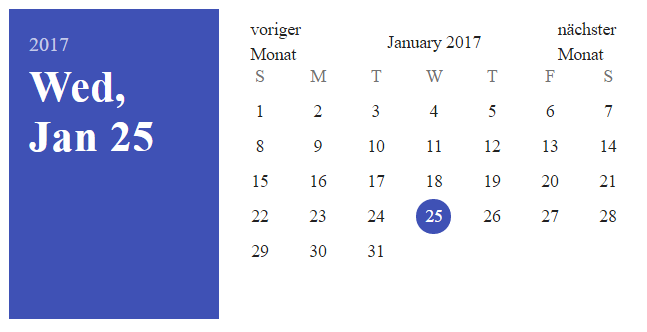
\includegraphics[width=0.7\textwidth,height=\textheight,keepaspectratio]{datPicErg.png}
		\caption[Adaptiver Paper Date Picker]{Adaptiver Paper Date Picker Web Component Ansicht Quelle: Bildschirmaufnahme des eigenen, vom Browser übersetzten, Programmcode}
		\label{img:datPicErg}
	\end{figure}\noindent
	Das Element wurde hier beispielhaft an einen Nutzer angepasst, dessen Präferenzwerte eine serife Schriftart und Text-Alternativen statt Symbole enthalten. 
	\newpage
	
	\section{Google Map}
	Zuletzt wurde das Element \enquote{google-map} ausgewählt. Es ist ein \emph{Web Component}, das die Anzeige einer \enquote{Google Map}, also einer Karte, ermöglicht \cite{gooMap}.
	\subsection{Konzeption zur Adaptivität}
	\label{ref:konVonAda}
	Abbildung \ref{img:gmap} zeigt die Ansicht einer \enquote{Google Map}. Sie nutzt einerseits farbige Abbildungen und Symbole, andererseits auch verschiedene Texte.
	\begin{figure}[H]
		\centering
		
\includegraphics[width=\textwidth,height=\textheight,keepaspectratio]{gmap.png}
		\caption[Google Map Web Component]{Google Map Web Component Ansicht \cite{gooMapGit}}
		\label{img:gmap}
	\end{figure}\noindent
	Um eine Adaptivität zu ermöglichen, sollte Einfluss auf den Kontrast, Text- und Symbol-Alternativen, die Schrift und die Leserichtung und damit auf die Anordnung der Elemente genommen werden. Der Kontrast der Kartenelemente sollte sich adaptiv an den Nutzer anpassen. Hier sollten die Straßen, Gebäude, Grünflächen und ähnliche Elemente, die durch Farbunterschiede dargestellt werden, sich stark voneinander abheben können, um allen Nutzern das Lesen der Karte zu ermöglichen. Des weiteren sollte sich die Schrift, also die Bezeichner der Kartenelemente, wie Städte, Straßen oder besondere Gebäude anpassen. Auch sollte sich die Schrift auf den Buttons einstellen lassen. Hier sollte es dem Nutzer ermöglicht werden zwischen einer kleinen, großen und einer serifen oder grotesken Schriftart zu wählen. Um sich an die Leserichtung des Anwenders anzupassen muss zum einen der Text und zum anderen der Aufbau des \emph{Web Components} sich verändern. So sollten das wichtigste Element, die Einstellungsleiste, sich bei einer Leserichtung von links nach rechts in der linken oberen Ecke befinden und bei einer Leserichtung von rechts nach links in der rechten oberen Ecke befinden. Dementsprechend würde sich der derzeitige, standardmäßige Aufbau der Karte bei einer Leserichtung von rechts nach links spiegeln. Zuletzt sollten für die Texte Text-Alternativen geboten werden und Bestandteile der Karte, die eine Funktion erfüllen und nur durch Abbildungen oder Symbole dargestellt werden, auch als Texte angeboten werden. 
	\subsection{Einrichtung des Google Map Web Component}
	Das \emph{Google Map Web Component} ist auf \enquote{GitHub} gespeichert \cite{gooMapGit}. Um die Möglichkeit zu erlangen es anzupassen wurde wiederum ein \enquote{fork} durchgeführt. Um die Abhängigkeiten des \emph{Web Component} zu installieren wurde \enquote{Bower} genutzt. Die \enquote{Google Map} selbst wird aus verschiedenen \emph{Web Components} zusammengesetzt. In der hier verwendeten Zusammenstellung werden die Elemente \enquote{google-map} und \enquote{google-maps-api} genutzt. Falls \enquote{Marker} gesetzt werden wird  auch das Element \enquote{iron-selector} genutzt. Wenn das \emph{Web Component} eingebunden ist, kann es unter dem \ac{HTML} \emph{Tag}  \enquote{<google-map>} genutzt werden. Dieses muss mit einem \enquote{Google} \ac{API} Schlüssel mit dem Namen \enquote{Google Maps JavaScript API} instanziiert werden. Dieser wurde über ein \enquote{Google} Benutzerkonto generiert und daraufhin in das \emph{Web Component} eingebunden. 
	\subsection{Umsetzung der Programmierung}
	Im weiteren wird die konzipierte Adaptivität des bestehenden \emph{Web Component} im Programmcode umgesetzt.
	\subsubsection{Kontrast}
	Zuerst wird die Anpassung des Kontrastwerts vorgenommen. Hier sollte zu Beginn auf die Erstellung einer \enquote{Google Map} genauer eingegangen werden. Dabei wird eine Instanz der Klasse \enquote{google.maps.Map} erstellt. Diese kann mithilfe optionaler Parameter erstellt werden. Einer dieser Parameter sind die sogenannten \enquote{styles}. Hier können einzelne Merkmale oder die gesamte Karte mit eigenen Gestaltungseinstellungen versehen werden. Ein Merkmal sind bestimmte geographische Eigenschaften der Karte, wie beispielsweise Straßen, Parks oder Seen, sie werden als \enquote{featureType} definiert. Danach können noch einzelne Elemente dieser Eigenschaften gewählt werden, wie beispielsweise Bezeichner oder geographische Elemente. Diese werden als \enquote{elementType} bezeichnet. Zuletzt kann das Aussehen dieser Elemente oder Merkmale über verschiedene Gestaltungsoptionen angepasst werden \cite{gmapStyle}.
\begin{listing}[H]
		\begin{JavaScriptcode*}{}
gmapstyles =
[
   {
      "featureType": "administrative",
      "elementType": "labels.text.fill",
      "stylers": [{
         "color": "#000000"
      }]
   },
   {
      "featureType": "administrative",
      "elementType": "labels.text.stroke",
      "stylers": [{
         "color": "#ffff00"
      }]
   },
   {
      "featureType": "landscape",
      "stylers": [{
      "color": "#000000"
      }]
   }
]
		\end{JavaScriptcode*}
		\caption[Anpassung zur Erhöhung des Kontrastwerts]{JavaScript Programmcode zur Gestaltung und Anpassung eines erhöhten Kontrastwerts}
		\label{lst:gooMapCon}
\end{listing}\noindent
In Listing \ref{lst:gooMapCon} ist ein Ausschnitt des Programmcodes der einen erhöhten Kontrast der Karte erreicht, dargestellt. Die hier erstellte Datengruppe wird als \enquote{styles} Parameter beim Instanziieren der \enquote{google.maps.Map} Klasse übergeben. Den Merkmalen der Karte werden verschiedene Farben zugeordnet, diese werden so gewählt, dass sie einen hohen Kontrast erzeugen und sich somit gut voneinander unterscheiden lassen. Diese Datengruppe soll jedoch nur verwendet werden wenn ein erhöhter Kontrast für den Nutzer erwünscht ist. Dafür wird dem \enquote{google-map} Element eine neue Eigenschaft \enquote{moreContrast} hinzugefügt. Diese ist vom Datentyp Boolean und der Standardwert ist \enquote{falsch}. Wird sie beim Einbinden des \emph{Web Component} gesetzt, wechselt ihr Wert auf \enquote{wahr}. 
Die Methode \enquote{\_getMapOptions} ist in dem Element \enquote{google-map} schon vor der Anpassung zur Adaptivität vorhanden. Diese erstellt eine Datengruppe \enquote{mapOptions}. Der wird die \enquote{styles} Datengruppe übergeben. Um eine Adaptivität zu ermöglichen wird hier der Datengruppe der Rückgabe-Wert der Methode \enquote{\_changeContrast} des \enquote{google-map} Elements übergeben. Diese fragt zu Beginn ab, ob die Eigenschaft \enquote{moreContrast} auf \enquote{wahr} gesetzt ist. Ist dies der Fall wird die vorher beschriebene Datengruppe für den erhöhten Kontrast an den \enquote{styles} Parameter übergeben, andernfalls wird der Standardwert überreicht. Somit wird insgesamt ein erhöhter Kontrast beim Setzen des Parameters \enquote{moreContrast} erreicht. 
	\subsubsection{Text-Alternativen}
	In einem adaptiven \emph{Web Component} sollte es ermöglicht werden, Symbole oder Abbildungen durch Texte darzustellen oder Texte durch Symbole zu ersetzen, falls dies möglich ist. In diesem \emph{Web Component} wird dafür die Methode \enquote{\_changeTextAlternatives} des \enquote{google-map} Elements verwendet. Diese wartet zu Beginn auf die Benachrichtigung des Ereignisses \enquote{idle} der \enquote{Google Map}. Diese bedeutet, dass alle Elemente der Karte nach einer Aktion wieder inaktiv sind. Dieses Ereignis wurde gewählt, da vor diesem Ereignis von der \enquote{Google Map} oft Änderungen zur Laufzeit entstehen und auf diese reagiert werden müssen. Danach fragt sie den Wert des Parameters \enquote{textAlternatives} ab. Dieser ist ein Parameter vom Datentyp \emph{String}. Wenn dieser Parameter den Wert \enquote{text} enthält, werden die Symbole der Kartensteuerung durch Text ersetzt. Die Steuerung der Vergrößerungsstufe erfolgt standardmäßig über ein Plus und ein Minus Symbol, wobei das Plus für Vergrößerung und das Minus für Verkleinerung steht. Diese werden durch die Texte \enquote{Vergrößern} und \enquote{Verkleinern} ersetzt. Da diese Texte je nach gewählter Schriftgröße eine unterschiedliche Breite und Höhe haben, siehe in nächstem Abschnitt \ref{sec:fontsize}, müssen die Größen der umgebenden Elemente angepasst werden. Diese bilden einen Rahmen um den Text oder ändern die Hintergrundfarbe der Texte. Dafür wird der Wert des Parameters \enquote{fontSize} abgefragt und dementsprechend die Höhe und Breite angepasst. Die Elemente der \enquote{Google Map} sind absolut positioniert. Deshalb läuft ein zu langer Text aus dem Sichtbereich des Nutzers oder überdeckt andere Elemente. Um dies zu unterbinden wird in der \enquote{\_changeTextAlternatives} Methode abgefragt, welche Leserichtung derzeit verwendet wird und aufgrund dieser Auskunft werden die Text-Alternativen so positioniert, dass sie immer komplett sichtbar sind. Das Symbol der kleinen Person für die Steuerung der \enquote{Street-View} Funktion kann nicht durch Text ersetzt werden. Da dieses Symbol mit der Maus auf eine bestimmte Stelle bewegt werden muss um die Funktion an genau dieser Stelle zu aktivieren, kann kein Text verwendet werden, da dieser zu breit wäre und die Stelle nicht eindeutig identifizierbar wäre. 
	\newline
	Ist der Wert des Parameters \enquote{textAlternatives} \enquote{symbol}, sollten alle Steuerungselemente die aus Text bestehen und durch Symbole ersetzt werden können, durch solche ausgetauscht werden. Dies trifft auf die Steuerung des Aussehens der Karte, die Elemente \enquote{Karte} und \enquote{Satellit} zu. Die Bibliothek \enquote{Font Awesome} wird als Quelle für die Symbole genutzt \cite{fonAwe}. Diese wird als eine Formatvorlage in die \ac{HTML} Seite geladen und einzelne Symbole können dann über \ac{CSS} Selektoren ausgewählt werden. Für die Einstellung Karte wird das Symbol \enquote{fa-map}, eine gefaltete Karte, genutzt und für die Einstellung Satellit das Symbol \enquote{fa-globe}, ein Globus. Diese werden dann bei Aufruf der Methode \enquote{\_changeTextAlternatives} des \enquote{google-map} Elements und einem mit \enquote{Symbol} versehenen Wert des \enquote{textAlternatives} Parameter gesetzt. Die Methode wird in die \enquote{\_initGMap} Methode hinzugefügt, hiermit wird erreicht, dass die Methode zur Adaptivität vom \emph{Web Component} selbst ausgeführt wird, denn die Methode \enquote{\_initGMap} wird in der \enquote{attached} \emph{Callback} Funktion der \enquote{Polymer} Bibliothek aufgerufen, wenn das Element an das \emph{document} angefügt wurde. Siehe mehr dazu in Kapitel \ref{sec:polLau}.
	\subsubsection{Schriftgröße}
	\label{sec:fontsize}
	Um die Adaptivität der Schriftgröße zu ermöglichen wird die Methode \enquote{\_changeFontSize} genutzt.  Sie wartet auch auf die Benachrichtigung des Ereignisses \enquote{idle} der \enquote{Google Map}. Daraufhin fragt sie den im Parameter \enquote{fontSize} gesetzten Wert ab. Anhand dieses Wertes werden Schriftgrößen für die verschiedenen Elemente der Karte gesetzt. Der Parameter \enquote{fontSize} kann die Werte \enquote{m},\enquote{l} oder \enquote{xl} enthalten. Von \enquote{m} bis \enquote{xl} werden die Schriftgrößen immer größer. Der Standardwert ist \enquote{m}, in diesem Fall wird die Schriftgröße nicht geändert. Danach werden die gesetzten Schriftgrößen auf die Kartenelemente übernommen. Darüber hinaus werden die Elemente bei Bedarf verschoben um ein sich gegenseitiges Überdecken dieser zu verhindern. Die Methode \enquote{\_changeFontSize} wird auch in die \enquote{\_initGMap} Methode eingefügt, um zu erreichen dass sie ausgeführt wird, wenn das Element an das \emph{document} angefügt wurde.
	\subsubsection{Schriftart}
	Die Schriftart kann sich auch an den Nutzer anpassen. Dies ermöglicht die Methode \enquote{\_changeFontStyle} des \enquote{google-map} Elements. Diese wartet auch auf die Benachrichtigung des Ereignisses \enquote{idle} der \enquote{Google Map}. Daraufhin wird abgefragt ob der Parameter \enquote{fontStyle} des \emph{Web Component} gesetzt ist. Ist dies der Fall wird der Wert des Parameters genutzt um die Schriftart der \enquote{google-map} auf eine serife oder serifenlose zu ändern. Eine Änderung findet nur statt wenn der Wert auf \enquote{serif} gesetzt ist, da im Standardzustand des \emph{Web Component} eine serifenlose Schriftart genutzt wird. Die Methode wird auch zur \enquote{\_initGMap} Methode hinzugefügt.
	\subsubsection{Leserichtung}
	Die Leserichtung des Nutzers hat primär Einfluss auf den Aufbau von Texten. Da dieses \emph{Web Component} nur einzelne Wörter enthält und keine ganzen Sätze, hat die Leserichtung in diesem Zusammenhang keine große Bedeutung. Jedoch hat sie einen Einfluss auf die Anordnung der Elemente. Die Methode \enquote{\_changeReadingDirection} des \enquote{google-map} Elements wartet auf die Benachrichtigung des Ereignisses \enquote{idle} der \enquote{Google Map}. Danach fragt sie den Wert des Parameters \enquote{readingDirection} ab und ändert die Anordnung der Elemente, falls dieser den Wert \enquote{rtl}, also Leserichtung von rechts nach links, enthält. Der Standardwert des Parameters ist \enquote{ltr}, standardmäßig ist die Anordnung der Elemente nach diesem Wert ausgerichtet. Da die \enquote{Google Maps} \ac{API} bei jedem Vergrößerungs- oder Verkleinerungs-Ereignis die Gestaltungseigenschaften der Elemente und damit ihre Anordnung im \emph{Web Component} neu berechnet, müssen die Auswirkungen der Leserichtung nach jedem Vergrößerungs- oder Verkleinerungs-Ereignis neu gesetzt werden. Deshalb wird auf das Ereignis \enquote{idle} gewartet und danach die Elemente, passend zur Leserichtung, wieder neu geordnet. Von dieser Änderung der Anordnung betroffen sind die beiden Schalter der Ansichtseinstellungen der Karte. Hier kann zwischen dem \enquote{Karte} und \enquote{Satellit} Wert gewählt werden. Darüber hinaus sind die Einstellungen der Vergrößerungsstufe und das Symbol der \enquote{Google Street View} von der Änderung betroffen. Auch die Methode \enquote{\_changeReadingDirection} wird zur Methode \enquote{\_initGMap} hinzugefügt.
	\subsubsection{Die adaptive Methode}
	Eine notwendige Besonderheit des \enquote{google-map} Elements ist die Abweichung der \enquote{adaptive} Methode. Jedes der zur Adaptivität erweiterten Elemente besitzt zwar diese Methode, jedoch besitzt sie in den anderen Elemente keine erweiterte Funktion, sondern zählt nur die zur Adaptivität benötigten Methoden auf und führt diese aus. In Listing \ref{lst:gmapAdaMet} ist der Programmcode dieser Methode dargestellt. In Zeile fünf bis acht werden, wie in den anderen erweiterten \emph{Web Components}, die Methoden zur Adaptivität aufgerufen. Die Abweichung dieser Methode beginnt jedoch schon in Zeile zwei. Hier wird der Kontrast-Wert gesetzt. Es wird abgefragt ob das \enquote{map} schon existiert.
		\begin{listing}[H]
		\begin{JavaScriptcode*}{}
adaptive: function(){
	if (this.map) {
		this.map.setOptions({styles: this._changeContrast()});
	}
	this._changeTextAlternatives();
	this._changeFontSize();
	this._changeFontStyle();
	this._changeReadingDirection();
	var thisMap = this.map;
	google.maps.event.trigger(thisMap, 'idle');
	google.maps.event.addListener(thisMap, 'tilesloaded', function(){
		setTimeout(function(){
			google.maps.event.trigger(thisMap, 'idle');
		}, 100);
	}.bind(this));
}
		\end{JavaScriptcode*}
		\caption[adaptive Methode der Google Map]{JavaScript Programmcode der Methode adaptive des google-map Elements}
		\label{lst:gmapAdaMet}
	\end{listing}\noindent
	Wenn dies der Fall ist, bedeutet das, dass die \enquote{styles} der Karte schon gesetzt werden. In diesem Fall werden die \enquote{styles} über die Methode \enquote{setOptions} neu gesetzt. Da die Methoden zur Adaptivität auf das \enquote{idle} Ereignis warten, wird nach dem Einbinden der Methoden, in Zeile zehn das \enquote{idle} Ereignis gesendet. Dadurch vollzieht das Element das erste Mal die Anpassung an die Präferenzen des Nutzers. Danach wird definiert, dass, wenn die Meldung \enquote{tilesloaded} eintritt, die Meldung \enquote{idle} nach einem sehr kurzen \emph{TimeOut}, also einer Wartezeit, erfolgen soll. Dadurch wird garantiert, dass die zur Laufzeit überschriebenen Werte auch nach dem Wechseln der Karten-Ansicht, also dem Wechsel zwischen der Satelliten- und der Karten-Ansicht, wieder an die Präferenzen der Nutzer angepasst werden. Die Wartezeit muss genutzt werden, da das Ereignis kurz vor der Anpassung zur Laufzeit durch die \enquote{google-map} erfolgt und somit sonst wieder überschrieben werden würde.
\newpage
\subsection{Beispiel-Ergebnis der Adaptivität}
In der Abbildung \ref{img:gmapErg} ist das adaptive \enquote{Google Map} Element  dargestellt.
\begin{figure}[H]		
	\centering
	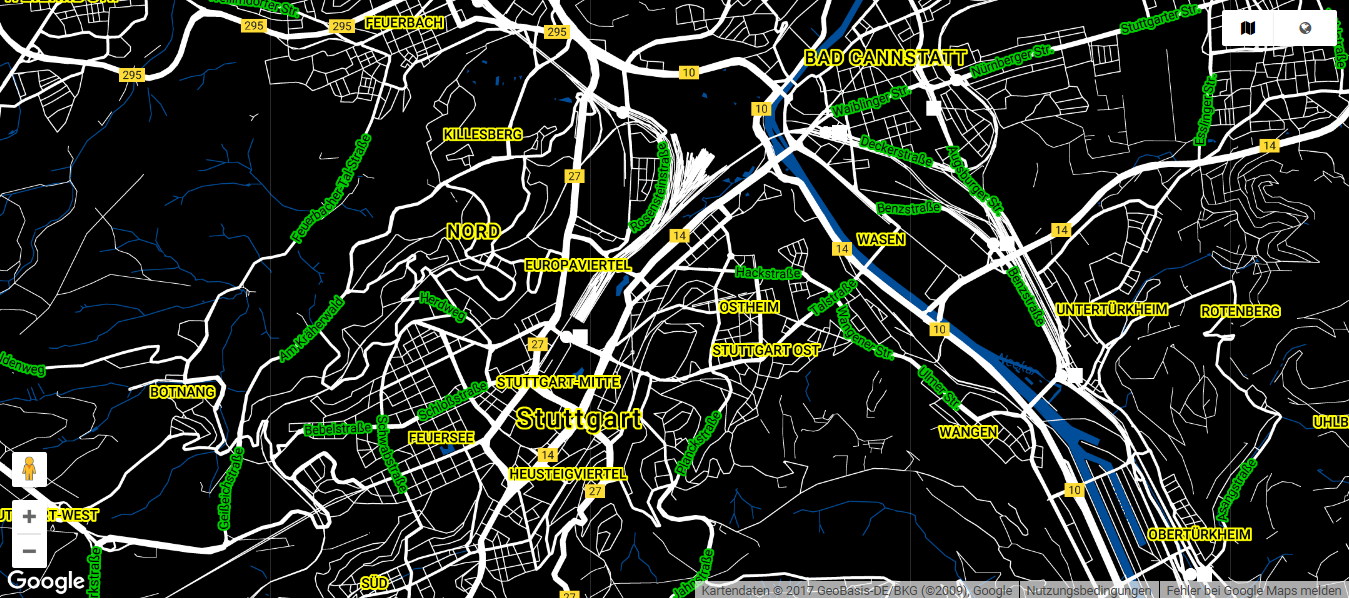
\includegraphics[width=\textwidth,height=\textheight,keepaspectratio]{gmapErg.png}
	\caption[Adaptive Google Map]{Adaptive Google Map Web Component Ansicht Quelle: Bildschirmaufnahme des eigenen, vom Browser übersetzten, Programmcode}
	\label{img:gmapErg}
\end{figure}\noindent
Das Element wurde hier beispielhaft an einen Nutzer angepasst, dessen Präferenzwerte einen erhöhten Kontrast, eine Leserichtung von rechts nach links und Symbol-Alternativen statt Texte enthalten. 
\newpage

\chapter{Evaluation der Adaptivitäts-Anpassungen}
Nachdem einige vorhandene \emph{Web Components}, realisiert mithilfe der \enquote{Polymer} Bibliothek, zur Adaptivität angepasst wurden, wird im folgenden darauf eingegangen, inwiefern die Adaptivität möglich ist und ob Hindernisse oder Möglichkeiten vorliegen.
	\section{Iron Data Table}
	\label{sec:evaIroDatTab}
	Eine Erweiterung zur Adaptivität ist möglich. Sie wird über das programmatische Hinzufügen von \ac{CSS} Klassen und der darauf folgenden Reaktion über Gestaltungsanweisungen realisiert. Je nach gewählter Präferenz werden verschiedene Klassen an die \emph{Web Components} angehängt und diese innerhalb der Komponenten genutzt um das Aussehen, den Aufbau oder den Inhalt anzupassen. Dies stellt jedoch das erste Problem dar. Jede Tabelle ist aus mehreren \emph{Web Components} zusammengesetzt. Es ist nicht möglich die Gestaltungsanweisungen in einer Komponente für alle Komponenten zu setzen, da \emph{Web Components} über den \emph{Shadow DOM} gekapselt sind. Somit können Gestaltungsanweisungen von einer Komponente keinen Einfluss auf eine andere Komponente nehmen. Deshalb müssen die Methoden zum Hinzufügen der \ac{CSS} Klassen in einer Komponente definiert werden, während die Methoden die Klassen auch zu anderen \emph{Web Components} hinzufügen müssen. Dies führt dazu, dass die Adaptivität nur vollständig gewährleistet ist, wenn die Zusammenstellung der verschiedenen \emph{Web Components} in einer bestimmten Form vorliegt. Zweitens müssen die Gestaltungsanweisungen zu jeder Komponente innerhalb dieser gesetzt werden. Dies führt dazu, dass der Programmcode der eine Adaptivität ermöglicht, auf verschiedene Komponenten und damit Dateien verteilt werden muss und somit schwerer wartbar ist. 
	\section{Paper Date Picker} 
	Auch die Adaptivität dieses Elements wird über das programmatische Hinzufügen von \ac{CSS} Klassen und eine Reaktion auf diese realisiert. Wiederum werden die Präferenzen des Nutzers anhand von \ac{CSS} Klassen an die Komponenten hinzugefügt. Hier entsteht dasselbe Problem wie im Kapitel \ref{sec:evaIroDatTab}, da der \enquote{Paper Date Picker} auch aus verschiedenen \emph{Web Components} besteht. So sind auch die Methoden zum Hinzufügen der Klassen in nur einer Komponente, die wiederum diese Klassen an andere Komponenten hinzufügen. Deshalb sollten die verschiedenen \emph{Web Components} in einer bestimmten Zusammenstellung vorliegen. Auch müssen die Gestaltungsanweisungen in jeder Komponente einzeln gesetzt werden was wiederum die Wartbarkeit mindert. Ein weiteres Hindernis zur Ermöglichung von Adaptivität dieser Komponente ist die Erstellung von Elementen zur Laufzeit. Die Komponente erstellt beispielsweise die Hintergrund-Farbänderung des derzeit ausgewählten Datums über das Hinzufügen der Klasse \enquote{selected} bei dem Auswählen dieses Datums. Das Aussehen dieses Elements, also nur dem gewählten Datum, sollte sich bei ermöglichter Adaptivität auch anpassen. Deshalb mussten hier neue Ereignisse erstellt und deren Meldungen abgewartet werden. Beispielsweise wird die Meldung \enquote{selectedDate} ausgegeben wenn ein Datum gewählt wird und bei erhöhter Kontrast-Präferenz des Nutzers diesem Datum die Klasse \enquote{moreContrast} hinzugefügt.
	\section{Google Map}
	\label{sec:fazGogMap}
	Die Anpassung zur Adaptivität dieses Elements ist problematischer.
	Es wird nicht alleine im \emph{Template} des \emph{Web Components} definiert, sondern zur Laufzeit bei der Initialisierung über die \ac{API} erstellt. Dies geschieht über die Methode \enquote{\_initGMap}. Hier wir ein neues \enquote{google.maps.Map} Objekt erstellt. Dieses erstellt die Elemente der Karte dann programmatisch. Dadurch liegt die Karte nicht von Beginn an vor, sondern wird erst zur Laufzeit der Applikation erstellt. Bei diesem Vorgang wird das Karten-Element auch über die \ac{CSS} Klasse \enquote{style-scope} gekapselt. Dies führt zu einigen Hindernissen. Zuerst führt die Kapselung dazu, dass Gestaltungsanweisungen keinen Einfluss auf Elemente innerhalb des Karten-Elements haben. Da auf den Programmcode des zur Laufzeit erstellten Karten-Elements, also der \ac{API}, kein Zugriff besteht und dieser deshalb  nicht verändert werden kann, können, im Gegensatz zu den in vorherigen Kapiteln beschriebenen \emph{Web Components}, keine \ac{CSS} Klassen zur Ermöglichung der Adaptivität genutzt werden. Die Gestaltungsanweisungen müssen zur Laufzeit über JavaScript erstellt werden. Ein weiteres Problem der Erstellung zur Laufzeit des Karten-Elements ist, dass die einzelnen Teile der Karte nicht beim ersten Laden der Internetseite vorhanden sind. So werden viele Elemente der Karte erst im Nachhinein nachgeladen und können nicht von Beginn an über JavaScript angesprochen werden. Deshalb müssen Ereignisse genutzt werden. Diese Ereignisse müssen abgewartet werden und erst nachdem die Meldung erbracht wird, dass sie vollzogen sind kann eine Methode zur Adaptivität ausgeführt werden. Die Karte wird jedoch nicht nur zur Laufzeit erstellt, sondern auch zur Laufzeit aktualisiert. So werden viele Gestaltungsanweisungen der Elemente der Karte bei verschiedenen Aktionen, beispielsweise dem vergrößern oder verkleinern, neu gesetzt oder überschrieben. Deshalb müssen diese Aktionen wieder über bestimmte Ereignisse und deren Meldungen abgewartet werden. Nachdem die Meldungen eintreffen und somit eine Aktion, welche die Komponente verändert hat, erfolgt ist, müssen die Gestaltungsanweisungen zu bestimmten Präferenzen der Nutzer wieder neu gesetzt werden. Zuletzt verwendet die zur Laufzeit erstellte Karte sehr wenig eindeutige Identifikatoren (Ids) oder \ac{CSS} Klassen. Dadurch ist es schwer, bestimmte Elemente eindeutig anzuwählen und mit diesen zu Arbeiten. Insgesamt ist es komplex das \enquote{Google Map} \emph{Web Component} zur Adaptivität zu erweitern, jedoch ist eine Adaptivität ermöglicht worden.
	

\chapter{Adaptive Web Components sind möglich}
Mithilfe von \emph{Web Components} ist eine kompakte Wiederverwendbarkeit von Komponenten möglich. Diese können beliebig oft und an verschiedenen Stellen von Webanwendungen eingesetzt werden. Diese Abhandlung führt zu dem Schluss, dass es insgesamt möglich ist diese zur Adaptivität zu erweitern. Dafür wird Programmcode innerhalb der Definition des \emph{Web Component} genutzt. In Kapitel \ref{sec:shaDowWebCom} ist dargelegt, dass diese Definition nur Einfluss auf diese eine bestimmte Art eines \emph{Web Component} hat, es kann bei richtiger Anwendung der Technologien ausgeschlossen werden dass Seiteneffekte von diesem auf andere Elemente einer Anwendung auftreten. Der Programmcode reagiert auf von außerhalb gesetzte Eigenschaften, die Präferenzen des Nutzers. Diese Präferenzen können in einer eindeutigen Art und Weise gespeichert werden, in der Form von \emph{Preference Sets}, um später die Eigenschaften der \emph{Web Components} zu bestimmen. Das Herunterladen dieser \emph{Preference Sets} erfolgt über einen \emph{REST-Call}, dargelegt in Kapitel \ref{sec:herPre}. Insgesamt können somit \emph{Web Components} über das Definieren von Methoden und Variablen erweitert werden, sich an die Präferenzen des Nutzers anzupassen. Dies Definition basiert auf dem Kapitel \ref{sec:adaVonBesWebCom}. Diese Anpassung zur Adaptivität erfolgt beim Aufruf einer Internetseite für jedes \emph{Web Component} einzeln und jedes dieser Komponenten kann beliebig oft in einer Internetseite eingebunden werden.
\newline
Jedoch ist eine lückenlose Adaptivität nur unter bestimmten Voraussetzungen möglich. Zuerst müssen die Präferenzen eindeutig definiert werden. Die Bezeichnungen der Präferenzen und auch die Werte dieser müssen eine allgemeingültige, also für jeden Nutzer gleiche, Bedeutung haben. Des weiteren müssen einige Konventionen bei der Erstellung von \emph{Web Components} beachtet werden. Erstens sollten einzelne \emph{Web Components} nicht aus zu vielen Komponenten zusammengesetzt werden. Wie in Kapitel \ref{sec:evaIroDatTab} dargelegt, muss die Erweiterung zur Adaptivität in jedem dieser Elemente einzeln definiert werden,  dies vermindert die Wartbarkeit und es können bei bestimmten Zusammenstellungen dieser einzelnen Komponenten ungewollte Seiteneffekte entstehen. Zweitens sollte möglichst die gesamte Komponente im \emph{Template} definiert werden und möglichst wenig zur Laufzeit erweitert oder verändert werden. Dadurch liegt das \emph{Web Component} zu Beginn im (möglichst) vollständigen Zustand vor und die Konzipierung zur Erweiterung zur Adaptivität kann das gesamte Elemente beachten. Wie Kapitel \ref{sec:fazGogMap} aufgezeigt, ist es problematisch wenn einzelne und insbesondere unterschiedliche Teile der Komponente zur Laufzeit nachgeladen werden, da diese die Definition von Adaptivität im Programmcode erschweren. Dieses Kapitel legt dar, dass Veränderungen zur Laufzeit bestimmte Anpassungen zur Adaptivität überschreiben und die Adaptivität annullieren können.
\newline
In der Zukunft der Webentwicklung könnte, wie in Kapitel \ref{sec:natBro} dargestellt, eine native Browser-Unterstützung der Technologien der \emph{Web Components} von allen modernen Browsern erfolgen. Dies würde dazu führen dass eindeutige und einheitliche Normen und \emph{Best Practices}, also eine Art Übersicht der besten Methoden und Praktiken, entstehen. Dies würde dazu führen dass Komponenten in ähnlicher oder gleicher Form definiert werden. Dadurch könnte die Definition von Adaptivität für viele verschiedene \emph{Web Components} einheitlich erfolgen. Der Programmcode zur Adaptivität müsste dann nicht extra für jede einzelne Komponente erstellt werden sondern könnte nur in einer Konfiguration angepasst werden. Eine wichtige Frage ist, ob die Adaptivität als eigene Eigenschaft oder Technologie in die \emph{Web Components} aufgenommen werden kann. Da die \emph{Web Components} immer wieder verschiedene Entwicklungen durchgemacht haben und verschiedene Technologien hinzugefügt oder herausgenommen wurden, wie dargelegt in Kapitel \ref{sec:dec}, ist es möglich dass die Adaptivität in Zukunft hinzugefügt wird. Dadurch würde der Aufbau von \emph{Web Components} so angepasst werden, dass eine Adaptivität leichter und konsistenter ermöglicht wäre. Eine konsistente Adaptivität von \emph{Web Components} wäre somit garantiert.
\printbibliography
\chapter*{Anhang}
\markboth{Anhang}{Anhang}
\addcontentsline{toc}{chapter}{Anhang}
Im Folgenden wird eine Übersicht der Daten auf der beigelegten CD gegeben. Die Ordnerstruktur setzt sich wie folgt zusammen.
\begin{enumerate}
	\item Programmcode
	\begin{enumerate}
		\item Globale Lizenz des erstellten Programmcodes
		\item Beispielprogrammcode
		\begin{enumerate}
			\item Genutzte Beispiele
				\begin{itemize}
					\item imports
					\item polymer
				\end{itemize}
			\item AWC
			\begin{itemize}
				\item assets
				\item comps
				\item lib
				\item spec
				\item src
			\end{itemize}
		\end{enumerate}
		\item Elemente zur Ermöglichung von Adaptivität
		\begin{enumerate}
			\item REST-client
			\item Preference Sets
		\end{enumerate} 
		\item Erweiterte Web Components
		\begin{enumerate}
			\item iron-data-table 
			\begin{itemize}
				\item bower\_components
				\item demo
				\item test
			\end{itemize}
			\item paper-date-picker
			\begin{itemize}
				\item bower\_components
				\item demo
				\item test
			\end{itemize}
			\item google-map
			\begin{itemize}
				\item bower\_components
				\item css
				\item demo
				\item test
				\item tmp
			\end{itemize}
		\end{enumerate} 
			\item Demonstrationswebseite
			\begin{itemize}
				\item bower\_components
				\item css
				\item imports
				\item javascript
			\end{itemize}
	\end{enumerate}
	\item Demonstrationsvideo
	\item GitHub Links
	\item Thesis
\end{enumerate}


	
\end{document}